\documentclass [12pt]{article}
\usepackage {nf,eqalign}
\usepackage{pdfpages}
\pagestyle{myheadings}
\topmargin -0.50truein
\oddsidemargin 0.truein
\textheight 9.00truein
\textwidth 6.5truein
\renewcommand{\baselinestretch}{1.5}
\parskip 0.10in

\def\u{{\bf u}}
\def\B{{\bf B}}
\def\E{{\bf E}}
\def\J{{\bf J}}
\def\v{{\bf v}}
\def\F{{\bf F}}
\def\R{{\bf R}}
\def\bx{B_x}
\def\curl{\nabla \times}
\def\div{\nabla \cdot}
\def\grad{\nabla}
\def\lap{\nabla^2}
\def\pt{\partial_t}
\def\pr{\partial_r}
\def\pz{\partial_z}
\def\bl{\item{$\bullet$}}
\def\sp{\item{-}}
\def\dz{{d \over dz}}
\def\rp{R^\prime}
\def\fc{{\cal F}}
\def\rc{{\cal R}}
\def\dec{\Delta {\cal E}}
\def\pd{\partial}
\def\deriv#1#2{{d#1\over d#2}}
\def\pderiv#1#2{{\partial#1\over \partial#2}}
\def\parder#1#2{{\partial#1\over\partial#2}}
\def\pardersq#1#2{{\partial^2#1\over\partial#2^2}}
\def\av#1{\left\langle#1\right\rangle}
\def\cosa{\cos \alpha}
\def\sina{\sin \alpha}
\def\epei{\epsilon_{e,i}}
\def\epnuie{\epsilon_{\nu i, \nu e}}
\def\vp{v_\perp}
\def\vh{\hat v}
\def\vhp{{\hat v}_\perp}
\def\epr{\epsilon_{\rho}}
\def\epd{\epsilon_{\Delta}}
\def\epl{\epsilon_{\lambda}}
\def\epnu{\epsilon_{\nu}}
\def\exb{{\bf E \! \times \! B}}
\def\iv{{\bf \hat i}}
\def\hsa{\hskip.4truein}
\def\hsp6{\hskip.6truein}
\def\hsm{\hskip.2truein}
\def\tild{$\sim$}
\def\la{$\langle$}
\def\ra{$\rangle$}


\title{Users Manual for the {\sf UEDGE} Edge-Plasma Transport Code}
\author{T.D. Rognlien, I. Joseph, W.H. Meyer, \\ M.E. Rensink, and M.V. Umansky \\
  Lawrence Livermore National Laboratory \\
  Livermore, CA 94551} 
\date{\today }
%%\date{LLNL Report: UCRL-ID-137121, Revised Oct. 17, 2002}

\begin{document}

\maketitle
\begin{flushleft}
   \texttt{LLNL Report No.: LLNL-SM-846481}
\end{flushleft}

\begin{abstract}

  Operational details are given for the two-dimensional {\sf UEDGE}
  edge-plasma transport code.  The model applies to plasma and neutral
  fluids in a strong magnetic field. Equations are solved for the
  plasma density, velocity along the magnetic field, electron
  temperature, ion temperature, and electrostatic potential.  In
  addition, fluid models of neutrals species are included or the
  option to couple to a Monte Carlo code description of the neutrals.
  Multi-species ion mixtures can be simulated.  The physical equations
  are discretized by a finite-difference procedure, and the resulting
  system of algebraic equations are solved by fully-implicit
  techniques.  The code can be used to follow time-dependent solutions
  or to find steady-state solutions by direct iteration.  The code is
  written in Fortran with a very small amount of amount C.  Calulations can be
  performed under Python or Basis code steering frameworks, which
  provide very similar functionality, with Python become the preferred
  method for new users.

%%\vskip1truein
%%\noindent
%%$^*$This work was performed under the auspices of the U.S.\ Department of
%%Energy by the University of California Lawrence Livermore National Laboratory
%%under contract No.~W-7405-Eng-48.
\end{abstract}

\tableofcontents


\pagebreak

\section{INTRODUCTION}

This report gives the operational details of how to use the {\sf UEDGE} code.
A brief description of the equations solved is included in the Appendix; for
more details, the reader can refer to the reference list at the end of this
report which include more information on the models and examples of the
results obtained with the code. The most up-to-date version of this manual
is available on the web site {\sf http://www.mfescience.org} and then opening
the links to Theory Group / Uedge Doc.

{\sf UEDGE} is a two-dimensional (2D) fluid transport code for collisional
edge plasmas.  Its primary use has been for tokamak edge plasmas in Magnetic
Fusion Energy devices, mainly tokamaks, although linear devices and spheromaks
have also been modeled.  {\sf UEDGE} typically generates a curvilinear mesh
based on the poloidal flux surfaces from an MHD equilibrium code such as {\sf
  EFIT} or {\sf TEQ}, but there are options for Cartesian meshes and
cylindrical meshes as well.

The basic physics equations are taken from Braginskii \cite{brag}, with the
addition of {\it ad hoc} anomalous or turbulence-enhanced transport
coefficients for the direction across the magnetic field; transport along the
magnetic field is taken as classical with flux limits.  A discussion of the
rationale for this procedure is given in Ref.~\cite{rog_ryu99}.  Also, an
arbitrary number of ion species can be included (limited by computer memory
and speed) which goes beyond Braginskii's model.  Line-radiation loss from
excitation, ionization, and recombination is incorporated into the electron
energy equation.  Neutral gas is described by fluid models or by coupling to a
Monte Carlo code.

At its inception in 1992, {\sf UEDGE} used a set of basic physics equations
and finite-differencing similar to that in the original {\sf B2} transport
code \cite{braams87,braams96}.  However, {\sf UEDGE} uses a fully implicit
procedure known as a modified Newton iteration to solve all of the equations
simultaneously rather the the semi-implicit {\sf SIMPLE} algorithm used in
{\sf B2}. Overviews of the fully-implicit method used in {\sf UEDGE} are given
in Refs.~\cite{brown86,saad96}. In addition, {\sf UEDGE}, now includes a
detailed fluid neutral model with a parallel momentum equation, calculation of
the electrostatic potential with $\exb$ and $\nabla B$ drift effects, and a
nonorthogonal mesh to conform to shaped divertor surfaces.  

References \citenum{r92a,r92b,p94,r94,s95,f95,p96,w96a,w96b,r96,r97,w97,r98a,r98b,re98,r99a,re99a,k99,r99} give many details of the models used in {\sf
  UEDGE} and some applications for edge-plasmas in fusion devices.  The list
is not intended to be exhaustive, but to serve as beginning bibliography for
those seeking more detail.

\section{Source Code, Variable Descriptor Files, and Building an Executable}

\subsection{Source code} \label{sourcsec}

The source code is maintained in a CVS archive on the MFE Program network at
LLNL. Precompilation processing can be done on any workstation that can access
to this network, and others can obtain the necessary files by contacting the
authors.  Compilation and loading is done on the machine where {\sf UEDGE} is
to be run.  Details of this procedure are given below in
Sec.~\ref{compilesec}.

{\sf UEDGE} is divided into ten {\sf BASIS} packages with different functions.
For example, the finite-differenced physics equations are contained in the
package {\sf bbb}, the grid generation routines are in packages {\sf flx} and
{\sf grd}, and the ({\sf pfb}) package (provided by {\sf BASIS} if used) allows
reading and writing data in a portable format PFB save file.  An alphabetical
list and summary of all of the packages (each having its own directory) and
several important auxiliary directories is as follows:

{\sf
\begin{tabbing} 
\hsa aph \hsp6\=  \# calculates atomic cross-sections for hydrogen \\
\hsa api     \> \# calculates atomic cross-sections for impurities \\
\hsa bbb     \> \# sets up the finite-difference physics equations and 
                                                              routines \\
             \> \# needed by the linear algebra solvers - the heart of UEDGE \\
\hsa com     \> \# contains routines and variables needed by various 
                                      packages \\
\hsa dce     \> \# distributed computing package - not generally needed \\
\hsa doc     \> \# documentation including UEDGE manual, uedge.man \\
\hsa dst     \> \# DUSTT module track/ablate dust; also idf,psi (UCSD) \\
\hsa idf     \> \# import data from file; used only by dst (DUSTT) (UCSD) \\
\hsa psi     \> \# plasma/surface interact; used only by dst (DUSTT (UCSD) \\
\hsa flx     \> \# calculates the magnetic flux surfaces for mesh \\
\hsa grd     \> \# calculates second mesh coordinate and constructs the mesh \\
\hsa in      \> \# various diagnostic routines (not a package) \\
\hsa ncl     \> \# NCLASS modular for neoclassical transport (ORNL)\\
\hsa scripts \> \# BASIS scripts for finding files (not a package) \\
\hsa svr     \> \# linear algebra and temporal integration routines \\
\hsa test    \> \# a few test cases (not a package) \\
\hsa wdf     \> \# calculates data needed by the DEGAS2 neutral M.C. code \\
\end{tabbing}
}

\subsection{Variables}

All of the variables within {\sf UEDGE}, together with a one-line description
of their meaning, are listed in files called the variable descriptor files
which are used in conjunction with either the {\sf BASIS} or {\sf PYTHON}
scripting systems that are used to drive/steer {\sf UEDGE}.  Generally, there
is one such file for each package listed above, with the name of the file
being {\sf package\_name.v} in the directory {\sf package\_name}.  For
example, variables for the physics equations and routines for the numerical
Jacobian in {\sf UEDGE} are included in the variable descriptor file called
{\sf bbb.v} in directory {\sf bbb}. In both {\sf BASIS} and {\sf PYTHON}
versions, all variables include the prefix from the package in which they are
defined, {\it i.e.}, most plasma physics variables have the {\sf bbb.} prefix.
However, an important difference between running under {\sf PYTHON} compared
to {\sf BASIS} is that {\sf PYTHON} requires you to use the prefix, whereas
{\sf BASIS} does not (although it allows prefixes to be used; if multiple
names exist and none is specified, it uses the name associated with the
package highest on the ``stack'', {\it i.e.}, most recently used).

The variables are combined into groups to make the process of identification
easier.  Also, if you know the name of the variable while running {\sf UEDGE},
at the {\sf UEDGE$>$} prompt, you may type {\sf list xyz}, and you will
receive the information about that variable included in the variable
descriptor file.  Also, if you know the name of the group, you can type {\sf
list groupname}, and receive a listing of that group from the variable
descriptor file.

The primary plasma fluid variables used in the code are as follows (where the
suppressed prefix of {\sf bbb.} must be used in the {\sf PYTHON} version, {\it
e.g.}, bbb.ni): 
{\sf
\begin{tabbing} 
\hsa ni(0:nx+1,0:ny+1,nfld)  \hsp6 \= Ion dens. [m**(-3)], nfld=species 
                                                         index (default=1)\\
\hsa up(0:nx+1,0:ny+1,nfld)  \> Parallel ion flow velocity [m/s]\\
\hsa te(0:nx+1,0:ny+1)       \> Electron temperature [Joules]\\
\hsa ti(0:nx+1,0:ny+1)       \> Ion temperature [Joules]\\
\hsa ng(0:nx+1,0:ny+1,ngsp)  \> Neutral gas density [m**(-3)], ngsp=species 
                                                                    index\\
\hsa phi(0:nx+1,0:ny+1)      \> Electrostatic potential [Volts]
\end{tabbing}
} 
%
Note that SI units (meters, volts, sec, {\it etc.}) are used throughout {\sf
UEDGE}, and scaling (normalization) is applied to the final ODE's and at the
linear algebra stage (row and column scaling). The first two indices for each
variable correspond to mesh indices {\sf (ix,iy)}, where {\sf ix} is the
poloidal index beginning at the inner divertor plate for a tokamak, and {\sf
iy} is the radial-like index beginning at the core boundary or the
private-flux-region wall.

The primary plasma fluid variables are used to evaluate the spatial
derivatives and source terms in the PDE's.  However, the variables that are
passed to the ODE and Newton solvers are somewhat different and normalized.
These are as follows:

{\sf
\begin{tabbing} 
\hsa For density:  \hsp6 \=  ni(i)/n0(i), where n0(i) is an input constant \\
\hsa For velocity:  \> ni(i)*up(i)/[n0(i)*cs], where cs is a constant 
                                                 ion-acoustic speed\\
\hsa For Te:        \> ne*te/(n0(1)*tnorm), where tnorm is a constant, 
                                                          ne = elec. dens.\\
\hsa For Ti:        \> ne*ti/(n0(1)*tnorm), where tnorm is a constant, 
                                                          ne = elec. dens.\\
\hsa For ng:        \> ng(i)/n0g(i)\\
\hsa For phi:       \> ev*phi/tnorm, where ev=1.6e-19 is the electron charge
\end{tabbing}
}

The conversion from plasma variables to ODE variables is done in
subroutine convrs; the reverse conversion is done by subroutine convert.

The ODE variables are stored in a 1-D vector call {\sf yl}, starting at ix=0,
iy=0.  The variables at that point are stored in the order listed above, then
the poloidal index, ix, is incremented until the ix=nx+1 boundary is reach,
then iy is incremented by unity, and the process repeated.  There are index
arrays that allow the user to determine the index ieq of {\sf yl(ieq)} that
corresponds to a variable at a given (ix,iy) location on the grid; these
arrays are defined as follows:

{\sf
\begin{tabbing} 
\hsa idxn(ix,iy,ifld): \hsp6 \=  yl ieq index for ni(i)/n0(i) \\
\hsa idxu(ix,iy,ifld):  \> yl ieq index for ni(i)*up(i)/[n0(i)*cs] \\
\hsa idxte(ix,iy):      \> yl ieq index for ne*te/[n0(1)*tnorm] \\
\hsa idxti(ix,iy):      \> yl ieq index for ne*ti/[n0(1)*tnorm] \\
\hsa idxg(ix,iy,igsp):  \> yl ieq index for ng(i)/n0g(i) \\
\hsa idxphi(ix,iy):     \> yl ieq index for ev*phi/tnorm
\end{tabbing}
}

There are also two arrays that the give the ix and iy indices for a given
{\sf yl} index ieq:

{\sf
\begin{tabbing} 
\hsa igyl(ieq,1):  \hsp6 \= ix poloidal index for ODE variable ieq  \\
\hsa igyl(ieq,2):  \> iy radial index for ODE variable ieq 
\end{tabbing}
}

\subsection{Compiling and loading a new executable} \label{compilesec}

The procedure for compiling and building the {\sf UEDGE} code is outlined
below: 

\noindent
Begin in your home directory, and un-tar the files containing {\sf UEDGE} by 
the command
\begin{verse} \sf
    tar xvf uedge\_Vx.x.tar 
\end{verse}
where Vx.x gives the {\sf UEDGE} version number.  See the Appendix
to correlate version numbers with dates.

Set the following environmental variables if you are using {\sf BASIS} to help
build and run {\sf UEDGE}: note that {\sf BASIS\_ROOT} and {\sf NCAR G\_ROOT}
will depend on where the system administrator has stored {\sf BASIS}, {\sf
NCAR} graphics, and {\sf PACT} (see {\sf http://pact.llnl.gov})on your
computer system
\begin{verse} \sf
 setenv UEDGE\_SCRIPTS \tild/uedge/scripts \\
 setenv BASIS\_ROOT /usr/local/nbasis \\
 setenv NCARG\_ROOT /usr/local \\
 setenv PACT /usr/local/pact \\
 setenv OPT '-native -03' \\
 set path = (\$BASIS\_ROOT/bin \$path)
\end{verse}
There are now two options for building {\sf UEDGE} with {\sf BASIS}, with the
preferred new method utilizing the {\sf MIO} system; the older method uses
{\sf MMM} as described in the next two subsections. 

If instead you are building the {\sf PYTHON} version of {\sf UEDGE}, most of
the required paths are set in the configure file
uedge/Python/config/ALL.config as described in more detail in
Sec.~\ref{pybuildsec}.  Pyuedge will run without using {\sf PACT} for creating
and reading {\sf PDB} format files for restart, but this is a very convenient
feature.  Thus, to use this option described below, you should install {\sf
PACT} (see {\sf http://pact.llnl.gov}), and continue to Sec.~\ref{pybuildsec}.

\subsubsection{Building {\sf UEDGE} for {\sf BASIS} with {\sf MIO}}
%
{\sf MIO} is now distributed with the {\sf BASIS} source code and needs to be
installed on your machine.  You can then learn some more about {\sf MIO} by
typing {\sf man mio}.  To build {\sf UEDGE}, go to the \tild/uedge/builder
directory and issue the following commands:
\begin{verse} \sf
   dsys config [-o] {\sf machine-dependent-file} \\
   dsys build \\
   dsys load \\
   dsys test 
\end{verse}
Here [-o] is the option to optimize (or -g for debug) and {\sf
  machine-dependent-file} is one of the file names in the builder/std
directory that contains {\sf MIO} switches appropriate for different computer
architectures, compilers, and options; for example, on {\sf linux} machines,
this file name often begins with (or is) {\sf linux}.  Thus, this is the file
that the user may need to edit for their specific machines.  The {\sf dsys
  test} command shown above runs a set of simple tests with the new executable
to confirm that the executable produces the same result for some base cases.
If there is a physics change or modification of the numerical scheme, the
reference pdb file needs to be updated in test/level\_2/ref directory; if this
pdb file is removed, the test script will properly add a new one after
obtaining the present solution.

The executable is located in \tild/uedge/dev/{\sf
  machine-dependent-name}/bin/xuedge.  Here {\sf
  machine-dependent-name}=lnx-2.1-i32, for example, on some LINUX machines.
The xuedge executable produced by {\sf MIO} should be functionally equivalent
to the executable produced the old way with {\sf MMM}, but it is stored in
a different location.

\subsubsection{Building {\sf UEDGE} under BASIS with {\sf MMM}}
%
Go to the \tild/uedge directory and issue the following to 
                                       generate the required make files 
\begin{verse} \sf
   mmm -ezn -rl 
\end{verse}
where ezn is the graphics package and rl is the readline library that
allows line editing and line recall. This command generates the makefiles
needed to compile and load {\sf UEDGE}.

\noindent
Finally, type the following line to compile and load the executable 
code {\sf xuedge}
\begin{verse} \sf
    gmake all xuedge 
\end{verse}
The excecutable {\sf xuedge} will appear in your uedge/LINUX directory if you
are on a LINUX system and more generally, in uedge/\$CPU.

\subsubsection{Building {\sf PYUEDGE} for use with {\sf PYTHON}}
\label{pybuildsec}
It is possible to build {\sf UEDGE} without {\sf BASIS}, but still having a 
scripting shell driven by {\sf PYTHON}.   Contributing to the development of
{\sf PYUEDGE} have sequentially been Dave Grote, Brian Yang, Tom Rognlien, 
and Lynda LoDestro. The only external source that you may need is the
preprocessor {\sf MPPL}, which converts the .m files of the {\sf UEDGE}
source code to {\sf FORTRAN} .f files.  The MPPL source and instructions can 
be obtained on the web from

{\bf http://w3.pppl.gov/rib/repositories/NTCC/files/mppl.tar.gz }

The {\sf UEDGE} source provides the {\sf Mac\_scripts} and {\sf PyMAC} scripts for
convert the variable descriptor files (.v) to {\sf FORTRAN}.  The content of this section is
included in updated form in the {\sf UEDGE} source file uedge/README\_Pyuedge, and
the user is encouraged to read this for any update differences to the following discussion.

To construct the PYTHON version of UEDGE, follow these steps:

{\bf Checking out and building the needed modules:}
\begin{enumerate}
%%    \begin{enumerate}
       \item If you have access to the LLNL/FEP cvs archives, then \\
       setenv CVS\_RSH=ssh  \\
       setenv CVSROOT :ext:$<$login-name$>$ \@hrothgar.llnl.gov:/usr/local/cvsroot
       \begin{enumerate}
           \item If BASIS is installed on the target computer, then \\
             cvs co [-P] pyUtils uedge \# -P empty dirs not checked out

           \item or, if BASIS is not installed, add Mac\_scripts to cvs co, i.e., \\
            cvs co [-P] pyUtils uedge Mac\_scripts \# -P empty dirs not checked out
      \end{enumerate}
%%    \end{itemize}

 \item or, if you get your copy of UEDGE from a tar file
  
   \begin{itemize}
      \item Set up a UEDGE directory and untar the file that should include the
         directories pyUtils, uedge, and Mac\_scripts(if BASIS is not on system)
   \end{itemize}
 %%\end{enumerate}
 
  \item Then, for either (1) or (2):
     \begin{enumerate}

       \item If BASIS is installed on your system (likely at LLNL, PPPL) then
   
       \begin{itemize} 
         \item Check that compiler paths, etc. are valid on your machine in the file  \\
           uedge/Pyuedge/config/*.config : Defaults are in config/ALL.config.
         \item Users must explicitly set the path variable {\sf TOPALL} in the file \\
               uedge/Python/Makefile to the parent directory of uedge and pyUtils \\
               directories
          \item 
            Then \\
              cd uedge/Pyuedge \\
              gmake make.all  \# builds pyUtils and Pyuedge
          
          \item A shared object file is produced as \\ uedge/Pyuedge/yoursys/uedge.so,
             where yoursys is the architecture variable ARCH, e.g., Linux
         \item To load uedge.so into a python session, startup python using the same
              version as defined in \\ 
              uedge/Pyuedge/config/\$(ARCH).config \\ 
              and read in the uedge startup script \\ 
              uedge/Pyuedge/uedge\_startup.py, i.e.
                 python \\
             $>>>$execfile('uedge\_startup.py')
         \end{itemize}

    \item If BASIS is not installed on your system
      \begin{itemize}
         \item MPPL must be installed first. MPPL can be downloaded from \\
           http://w3.pppl.gov/rib/repositories/NTCC/catalog
         \item Check the directory structure from (1) or (2) above; must include 3
           directories: pyUtils, uedge, and Mac\_scripts
         \item Check that compiler paths, etc. are valid on your machine in the file \\
           uedge/Pyuedge/config/*.config : Defaults are in config/ALL.config.
         \item Users must explicitly set the path variable {\sf TOPALL} in the file \\
               uedge/Python/Makefile to the parent directory of uedge and pyUtils \\
               directories
         \item Then \\
           cd uedge/Pyuedge \\
           gmake make.all  \# builds pyUtils and Pyuedge
          \item A shared object file is produced as uedge/Pyuedge/yoursys/uedge.so,
             where yoursys is the architecture variable ARCH, e.g., Linux
         \item To load uedge.so into a python session, startup python using the same
              version as defined in \\ 
               uedge/Pyuedge/config/\$(ARCH).config \\ 
              and read in the uedge startup script \\ 
                uedge/Pyuedge/uedge\_startup.py, i.e. \\
                 python \\
                  $>>>$execfile('uedge\_startup.py')
         \end{itemize}
  \end{enumerate}
   \item  Additional useful commands/information \\
   Other gmake commands:
     \begin{itemize}
       \item gmake           \# builds only Pyuedge
       \item gmake clean     \# cleans only Pyuedge
       \item gmake clean.all \# cleans both pyUtils and Pyuedge
     \end{itemize}
     
  Key make-variables for customizing directory locations:
  \begin{verse} 
   CONFIG   - path to the config directory. It is set in Pyuedge/Makefile \\
   PYUTILS  - path to the pyUtils directory. It is set Pyuedge/Makefile
              (overrides the default, which is set in config/ALL.config) \\
   HasBASIS - determines which mac and mppl are used;
              defaulted in config/ALL.config. \\

           \noindent  If HasBASIS is defined, the following must be set:\\
   BASIS\_ROOT  - path to basis; mac and mppl from basis are used.\\

           \noindent If HasBASIS is undefined, the following are needed:\\
   MAC         - The mac utility executable; defaulted in config/ALL.config.\\
   MPPL\_ROOT   - path to MPPL. There is no platform-independent default
                 set up (gmake will crash if MPPL\_ROOT is not found).\\
   PYTHON\_ROOT, PYVERS - path and python version\\
  \end{verse}

Compiler, etc., paths and options are defaulted in config/ALL.config. The
platform-dependent settings are in the appropriate config/*.config file.
\end{enumerate}

To run a simple test case (which automatically reads in 
    uedge/Pyuedge/uedge\_startup.py), do the following in uedge/Pyuedge
    \begin{verse}
      python \\
      $>>>$execfile('rdtest\_linux.py')
    \end{verse}
    
The session should look something like the following: \\
hrethric:rognlien(LINUX)$>$ pyuedge \hfil\break
Python 2.2 (\#3, Mar 11 2002, 13:29:17)\hfil\break
[GCC 2.96 20000731 (Red Hat Linux 7.1 2.96-85)] on linux2\hfil\break
Type "help", "copyright", "credits" or "license" for more information.\hfil\break
$>>>$ execfile('rdtest\_linux.py')\hfil\break

You type the last line to read the file rdtest\_linux.py, which contains input
parameters and the call to the driver routine bbb.exmain.  This case solves
for four plasma variables (density - bbb.ni, parallel velocity - bbb.up,
electron temperature - bbb.te, and ion temperature - bbb.ti), which are
advanced time-dependently, nearly to steady state.  The four variables are
printed at the end of the run.  Also note that to execute {\sf UEDGE} under
{\sf PYTHON}, that you must call the subroutine {\sf exmain} as bbb.exmain().

Note that in PYTHON, all variables and subroutines carry the name of the
package with which they are associated, e.g., the ion density is bbb.ni(ix,iy)
rather than just ni(ix,iy) in the BASIS version.  In fact, BASIS also names ni
$\rightarrow$ bbb.ni, but the bbb. is suppressed unless the user explicitly
includes it in commands.

Also note that rdtest\_linux.py has an initial command
execfile('uedge\_startup.py') that reads the file uedge\_startup.py, which
imports the required packages into the pyuedge session.

\noindent Again be sure that the python version you run here is the same version as
was used in the build ( $(PYTHON\_ROOT)/bin/python$(PYVERS) ), where 
PYTHON\_ROOT and PYVERS are as defined in your 
uedge/Pyuedge/config/*.config file.

To modify uedge sources and recompile, note that there
is no uedge source-code under uedge/Pyuedge except for the
file Pyuedge/Fsor/ex\_das\_isa.f. Make changes in the uedge source-code
directories parallel to Pyuedge, {\it e.g.} uedge/bbb or uedge/com, {\it etc.}; 
then return to Pyuedge and type gmake.

\section{Basic Mechanics of Code Execution}
\subsection{Reading input and execution}

(Note: this section was written to describe running {\sf UEDGE} under {\sf
BASIS} although the basic steps have close counterparts when using the {\sf
PYTHON} version.)

The executable for {\sf UEDGE} is typically called {\sf xuedge}, or sometimes
just {\sf uedge} on NERSC machines.  The build and loading procedure is
described in Sec.~\ref{compilesec}, which results in the executable being
found in {\sf \tild developer/uedge/SOL}, where developer is the name of the
person who created the executable and SOL refers to the SUN Solaris system.
On other workstations, SOL will be replaced by something like HP700 for HPs or
AXP for DECs, etc.

Before running the {\sf BASIS} version of {\sf UEDGE}, or {\sf xuedge}, you
need to set two environmental variables if you have not already done so for
the compilation and loading of {\sf UEDGE} described in Sec.~\ref{compilesec}.
If you are running on the LLNL MFE SUN solaris system, you can just set two
environmental variables: {\sf UEDGE\_SCRIPTS} to {\sf
/home/rognlien/uedge/scripts} and {\sf UEDGE} to {\sf /home/rognlien/uedge}.
Then you need not worry about the {\sf aphdir} and {\sf uedge\_path} files. If
you are on another system, or want to read your own atomic physics and script
files, place the contents of {\sf uedge/in/aph} and {\sf uedge/in/api} in some
directory, and then set the environmental variable {\sf UEDGE} to point to
them.  Likewise, copy and then change what is in {\sf uedge/scripts} and set
up the environmental variable {\sf UEDGE\_SCRIPTS} to point to that directory.

The {\sf aphdir} file tell {\sf UEDGE} where to locate the hydrogen atomic
rate files, and on the LLNL MFE SUN solaris system, it should contain the line

\begin{verse} \sf
aphdir = ``/mfe/theory/Uedge/Ver\_XX/uedge/in/aph"
\end{verse}
where the {\sf XX} is the most current version number shown in the Uedge
directory.  The second file, {\sf uedge\_path}, tells {\sf UEDGE} where to
find various diagnostic files.  Again, on the LLNL MFE SUN solaris system, it
should contain the line

\begin{verse} \sf
call pathadd(``/mfe/theory/Uedge/Ver\_XX/uedge/in")
\end{verse}
%
One can add other lines to tell {\sf UEDGE} to search other paths (directories)
in response to a command issued from the parser.

If you are running the {\sf PYTHON} version of {\sf UEDGE}, you need to set
the character variable {\sf aph.aphdir} in your input file to the path of the
directory containing the hydrogen atomic data.  For example, this may be

\begin{verse} \sf
aph.aphdir = ``/mfe/theory/Uedge/Ver\_XX/uedge/in/aph")
\end{verse}

To run a case, simply type {\sf xuedge} (or {\sf uedge} if you are using the
public version on the NERSC system).  The executable will then automatically
read a default input file called {\sf .basis}, if it exists in the directory
(generally not used, however).  After {\sf UEDGE} has read the {\sf .basis}
file, it comes back with the prompt {\sf UEDGE$>$}, at which point you need to
type a command.  Typically, you will read a second file which contains the
input settings for various control variables and switches; we usually use the
convention that such input files begin with the letters rd (which stands for
``read"), but this is not necessary.  Thus, you will type something like {\sf
  read rddata2}. You may also start the executable and read the input file on
a single line with the command {\sf xuedge read rddata2}.  Some example files
can be found in the location noted below in Sample Problems section. You can
also change any variable at the prompt by typing, say, runtim=1.e-10, to
modify runtim.

Once all the variables have been set, you execute the code by typing {\sf
  exmain}.  What this does is tell the {\sf BASIS} system to execute the
subroutine named {\sf exmain}, which calls all the appropriate subroutines to
execute a full run.  It is also possible under {\sf BASIS} to call other
subroutines independently, but this is usually only done for debugging
purposes.  Thus, a typical session with {\sf UEDGE} will look as follows:
\begin{verse} \sf
xuedge\\
UEDGE$>$ read rddata2\\
UEDGE$>$ exmain\\
UEDGE$>$
\end{verse}
The last prompt means the code has successfully completed the run and is ready
for more input.  If you want to stop, just type {\sf end}.  You can also
display the results without exiting from the {\sf BASIS} session.
 

\subsection{Sample problems}

There are a set of sample problems that can be run.  For example, on the LLNL
MFE LINUX system, one can go to the directory {\sf
  \tild rognlien/uedge/Applic/Examples}.  It is best to check with one of the
current users to learn more details of these examples.  Note that these examples
pertain to running {\sf UEDGE} under {\sf BASIS}, but there is a very close
correspondence to running under {\sf PYTHON}.
 
\subsection{Displaying results}

You may want to list any variable or array to see what the solution looks
like.  For example, the 2-D electron temperature is stored in the array {\sf
  te(0:nx+1,0:ny+1)} in units of Joules.  You may specify the number of places
to be displayed after the decimal point by typing {\sf fuzz=2}, for example.
Thus, the following sequence will print out the electron temperature array in
electron volts:
\begin{verse} \sf
fuzz=2\\
te/ev
\end{verse}
where ev=1.6e-19 Joules/eV is a variable in the code for converting from
Joules to electron volts.  If you want to list some other variable to 4
decimal places you must first type {\sf fuzz=4}, which will hold until another
{\sf fuzz=} statement is typed.

You can also do plots of arrays to look at the present solution.  To plot the
function y(x), type {\sf plot y,x}.  To do a contour plot of z(x,y), type {\sf
  plotz z,x,y}.  

All of the commands useable at the {\sf UEDGE$>$} prompt are in the {\sf
  BASIS} command language, which is extensive and powerful yet easy to learn.
The {\sf BASIS} manual can be read and searched with a web browser (see the
URL {\sf http://xfiles.llnl.gov/basis/}).  The plotting package {\sf EZN} is
  also part of {\sf BASIS}.

\subsection{Instantaneous output and run termination}

While running a time-dependent problem with any solver (except {\sf lsode},
which is not a currently supported option), you may obtain information on the
present status of the solution by typing {\sf s} or {\sf status} and a return.
In order to do this, you must first set the switch {\sf iskaboom=1}; this
option does not work on some platforms - notably, PCs running LINUX and
possible others.  If the code appears to ``hang'' without doing anything, one
cause can be {\sf iskaboom=1} on a platform that will not support this
options; try setting {\sf iskaboom=0}.  Also, if you run {\sf xuedge} in the
background, you need to set {\sf iskaboom=0}.  

If {\sf iskaboom=1} and you type {\sf s}, you will receive lines of output
giving the total number of function and preconditioner evaluations, nfe and
npe, respectively, and the {\sf yl} index {\sf ieq} (imxtstep) of the equation
that is restricting the time step.  A second index, imxnewt, gives the {\sf
  ieq} of the equation that is requiring the Jacobian to be reevaluated, if
that is limiting the time step.  In addition, it gives the total simulation
time and the present time step, {\sf dt}.  A third line gives detail data on
the error estimates from the ODE solver: {\sf bigts} is for the time
integration and {\sf dsm} is for the Jacobian.

If you want to abort the present simulation and return to the {\sf UEDGE$>$}
prompt, type ctrl-c and a return. At this point, {\sf BASIS} with give the
prompt DEBUG$>$; you now may query {\sf UEDGE} for variable values, etc., and
then type {\sf cont} if you want to continue the calculation.  If you type
{\sf abort}, to the DEBUG$>$ prompt, you will return to the {\sf UEDGE$>$}
prompt.  You can do this for DEBUG$>$ during either a time-dependent solution
or a Newton iteration.  If you then restart after changing some parameters,
the code initializes itself as though the aborted run had not taken place.

\subsection{Restarting from present solution}

If you are still in an active {\sf BASIS} session, you can set restart=1 to
use the present solution as initial conditions for the next execution.  You
can also double the grid in both x and y directions by being sure that
newgeo=1, restart=1 and by doubling {\sf nxleg, nxcore, nycore, nysol,} and
{\sf nxomit}.  The present solution is then interpolated to the finer grid as
the initial conditions for the new run.  This is conveniently done by reading
a file called {\sf double} with {\sf BASIS} (i.e., type {\sf read double})
that has the necessary parameter adjustments in it. You can double the mesh
separately in the radial or poloidal direction, or incrementally; see
Sec.~\ref{interpsec} for more details.

\subsection{Creating and restarting from a {\sf BASIS} portable PFB save file}

{\sf BASIS} has a very useful facility to save any variables you wish to a
portable file that can be read in a subsequent session.  To do this, type {\sf
  create sfile}, where sfile is some name you choose for the data file.  Then
you can save any variables you want by typing {\sf write x,y,te}.  This
command can be repeated; to stop the writing to this file, type {\sf close}.
The minimum data set you must save in a portable file to make a restart is the
set of plasma variables; you should also save any special variable settings.
An example for the minimum saving procedure is as follows:

\begin{verse} \sf
create stest1 \\
write nis,ups,tes,tis,ngs,phis \\
close
\end{verse}
%
{\sf UEDGE} uses the convention that the plasma variables used for restarting
all have the letter ``s" appended to them.

To use the portable file, you must be sure that you have the same grid size
as that of the saved data.  You then execute {\sf UEDGE} as for a normal run by
reading input files (but don't type {\sf exmain} yet).  Then give the following
commands:

\begin{verse} \sf
allocate \\
restore stest1 \\
restart=1
\end{verse}
%
Here, allocate generates the appropriate arrays through dynamic allocation.
At this point, one may type {\sf exmain} to begin the run with the values
saved previously in stest1.  It is convenient to save the final state of
converged runs in case you want to restart from them at some later date.
Also, the portable files can be moved (using the binary mode of {\sf ftp}) to
computers using different numerical representations and used to continue runs.

Before version 10.0 of {\sf BASIS}, a capability was present to create
savefiles using commands {\sf save to}, {\sf save}, and {\sf save off}; users
of more recent vesions do not need to concern themselves with this difference.
The portable file capability (PFB or PDB) should be used now to create new
files, but the user may want to use a version of {\sf UEDGE} created with
version 9.11 of {\sf BASIS} to convert from the savefile format to the \\ \\
portable format.  Use the {\sf readb} command to read a savefile just as you
would use {\sf restore} to read a portable file.  Then use {\sf create}, {\sf
  write}, and {\sf close} to save the data in a portable file.

\subsection{Creating and restarting from a {\sf PYTHON}-based portable PDB save file}

If you are using {\sf PYUEDGE} rather than the {\sf BASIS} version,
you can still create and restore saved solutions from PDB files.  To
do so, you need to have installed libraries associated with {\sf PACT}
and the scripts from {\sf PyPDB}.  Information in this section came
from Dave Grote, LBL.  {\sf PACT} is a suite of tools developed at
LLNL that allows creating and reading self-describing pdb data files
(as used by {\sf BASIS} above).  {\sf PACT} can be found at
{\sf http://pact.llnl.gov}.  {\sf PyPDB} are scripts that give
{\sf PYTHON} access to these tools.

After installing {\sf PACT} and {\sf PyPDB}, the user can create a {\sf PDB} save 
file under a pyuedge session as follows:
  \begin{verse} \sf
    ff = PW.PW("pf\_case1") \\
    ff.nis = bbb.nis \\
    ff.ups = bbb.ups \\
    ff.tes = bbb.tes \\
    ff.ngs = bbb.ngs \\
    ff.phis = bbb.phis \\
    ff.close()
  \end{verse}
  
To read such a file back into {\sf PYEDGE}, the user can type
  \begin{verse} \sf
    restore('pf\_case1')
  \end{verse}
  
  \noindent  (single or double quotes should work), or
  
  \begin{verse} \sf
     ff = PR.PR("pf\_case1") \\
     bbb.nis = ff.nis \\
     bbb.ups = ff.ups \\
     bbb.tes = ff.te \\
     bbb.tis = ff.ti \\
     bbb.ngs = ff.ng \\
     bbb.phis = ff.phi \\
     ff.close()
  \end{verse}
  
\subsection{Interpolating the solution to a new mesh and restarting}
\label{interpsec}

{\sf UEDGE} has three different linear interpolating options; these are
controlled by the switches {\sf isnintp} and {\sf isgindx}. If {\sf
  isnintp=0}, {\sf isgindx} is immaterial, and the ``old" interpolator is used
that only allows the users to double the mesh in each direction. That is, if
you are starting from a solution with a certain set of grid indices {\sf
  nxleg(1,1), nxleg(1,2), nxcore(1,1), nxcore(1,2), nysol(1),} and {\sf
  nycore(1)}, you must double all of these. This interpolation is rather crude
in that it assumes the mesh is uniform in each direction, but it works
surprisingly well. However, doubling the mesh in each direction is sometimes
too large a change for the Newton method to converge on the finer mesh. The
next two methods allow an arbitrary change in the number of mesh points.

If {\sf isnintp}=1 the user may increase or decrease the mesh by any amount in
either direction. For this case, two options are available: {\sf isgindx}=1
and 0.  For {\sf isgindx}=1 (default and recommended setting), the
interpolation occurs in index space as though the mesh is uniform. This case
is thus similar to the {\sf isnintp}=0 option discussed above.  However, there
is a difference (other than the arbitrary mesh change) in that here values are
not interpolated across the separatrix or across the radial cut through the
x-point, but are rather extrapolated at these locations. The reason for doing
this across the separatrix is that linear interpolation often does a poor job
because of the abrupt change in variables there; it is done across the radial
cut only for simplicity of the algorithm. Treating the region above and below
the separatrix independently (and on either side of the cut) allows one to add
extra mesh points in either region without perturbing the other.

For isnintp=1 and isgindx=0, the code does a linear interpolation using the
actual (normalized) mesh which is not uniform or rectangular. This scheme does
not seem to outperform the simpler index-based algorithm, and sometimes has
trouble finding the appropriate mesh points for performing the interpolation.
The message {\sf ***** grdinty cannot find straddling grid...} is printed if
the algorithm fails to find the appropriate mesh points. In that case, switch
to {\sf isgindx}=1.

It is possible to interpolate from a save-file solution, even if the code does
not converge to this case first. One needs to generate the old mesh and then
type {\sf call gridseq} from the {\sf UEDGE} prompt (the {\sf BASIS} parser).
Alternatively, use a very loose tolerance for {\sf svrpkg=``nksol"}, say {\sf
ftol}=1.e10, so the code will think it has converged after one iteration. The
mesh may then be changed without any extra call to {\sf gridseq}.


\section{Grid Generation}

\subsection{Mesh generation using MHD equilibria}
The grid generated in {\sf UEDGE} uses routines that are an extension and
modification of a grid generator developed by M. Petravic at PPPL
\cite{petravic87}. Data on the location of poloidal magnetic flux surfaces are
generated by one of various MHD equilibrium codes ({\it e.g.}, {\sf TEQ,
  EFIT}), and then read into {\sf UEDGE} via two files. These files must be
named {\sf aeqdsk} and {\sf neqdsk}, and the switches {\sf mhdgeo}=1 and {\sf
  gengrid}=1 must be set.  If {\sf gengrid}=0, {\sf UEDGE} reads in a file
with the grid information already in it called {\sf gridue}. The {\sf gridue}
file can be generated by a previous {\sf UEDGE} run. For large problems,
precomputing the {\sf gridue} file and using {\sf gengrid}=0 can save
considerable storage. One can generate the grid in {\sf UEDGE} without running
a complete problem; just type
\begin{verse} \sf
      call flxrun \\
      call grdrun
\end{verse}
and the file {\sf gridue} will be generated. This call sequence is done
automatically if you execute a full problem by typing {\sf exmain}.

There are a number of configuration options available for grid
generation with {\sf mhdgeo}=1; we mention a few here.
Set {\sf geometry=``snull''} for lower-single-null configurations; if there
is a secondary (upper) x-point, the outermost flux surface will be
adjusted by the code so as to exclude the second x-point.
Set {\sf geometry=``uppersn''} for upper-single-null configurations; in this
case the observer reference frame is simply tranformed so the
configuration appears as a lower-single-null.
Set {\sf geometry=``dnbot''} to generate a half-mesh that contains a lower
x-point and a symmetry boundary at the midplane; this option can be
used with any eqdsk that contains a lower x-point (either lower
single-null or double-null configurations).
Set {\sf geometry=``dnull''} to generate an up/down symmetric double-null mesh
that includes both x-points; the lower half-mesh (as decribed above
for {\sf geometry=``dnbot''}) will be exactly duplicated in the upper half to
form the complete mesh; this option can be used with any eqdsk that
contains a lower x-point (either lower single-null or double-null
configurations).
To generate a mesh that includes both x-points of a non-symmetric
double-null configuration, one generates separate meshes for the upper
and lower halves (as in {\sf geometry=``dnbot''}), and combines these to form a
complete mesh for the configuration; see the example given below.

The construction of a full double-null mesh is illustrated in the script
 {\sf makemesh\_dRsep\_m1} and associated files.  These files
are stored in the {\sf uedge/test/rensink/dnull} subdirectory of the {\sf UEDGE}
source code distribution.  This example uses a very small number of
grid points to more clearly exhibit certain features of the mesh; for
a realistic simulation one would use much finer resolution in both the
radial and poloidal directions.  The construction procedure consists of the following eight steps which
are identified in the script that implements this example:
\begin{enumerate}
\item read the eqdsk to identify x-points and separatrices
\item specify the radial distribution of flux surfaces
\item construct the mesh for the upper half of the configuration
\item construct the mesh for the lower half of the configuration
\item combine the two halves of the mesh
\item define guard cells at the divertor target plates
\item compute magnetic field values for each cell
\item write out the {\sf gridue} file
\end{enumerate}
It is important to note that for any up/down asymmetric double-null
configuration, the radial mesh option {\sf kymesh}=0 MUST be used.  Also,
steps 3 and 4 can be modified to create either orthogonal or
non-orthogonal meshes, as desired.

It is also
possible to simulate the outer half of a single null or the lower, outer
quadrant of a double null where reflection boundary conditions are used at the
left boundary and no flux is allowed through the outer (ix=ixpt2) cut at the
x-point. To do this latter type of geometry, set these variables: {\sf
\begin{tabbing}
\hsa nxomit      \hsa\= \# Number of poloidal grid points to omit before 
                                                            setting\\
                 \> \# reflection boundary condition. Files double, etc.\\
                 \>  \# automatically change nxomit to correct value\\
\hsa isfixlb = 2 \>  \# Sets reflection bc at ix = nxomit and no-flux bc at\\
                 \>  \# ix = ixpt2 (outer x-point cut)
\end{tabbing}
}
The radial distribution of the mesh is controlled by the following
input parameters.  The poloidal flux, psi, is normalized to be unity
on the separatrix and the radial boundaries of the mesh are specified by:
{\sf
\begin{tabbing}
\hsa psi0min1  \hsa\=  :flux at the inner core boundary, 0.98 is typical\\
\hsa psi0min2       \>  :flux at the private-flux region boundary, 0.98 
                                                               is typical\\
\hsa psi0sep        \>  :flux very near the separatrix, use 1.00005\\
\hsa psi0max        \>  :flux at the outer wall boundary, 1.07 is typical
\end{tabbing}
}
The number of radial cells in various regions is:
{\sf
\begin{tabbing}
\hsa nycore(1) \hsa\=  :number of radial cells in core (and private-flux) 
                                                                 region\\
\hsa nysol(1)        \> :number of radial cells in scrape-off layer
\end{tabbing}
}
The radial distribution of mesh flux surfaces is controlled by the
input parameter {\sf kymesh}.  For {\sf kymesh}=1 (the default value) analytic forms are used to radially
distribute the normalized flux values between {\sf psi0min} and {\sf psi0sep}, and
between {\sf psi0sep} and {\sf psi0max}; the input variable {\sf alfcy} provides some
additional control over the radial distribution.  One can cause the
flux surfaces to cluster near the separatrix by making the variable
alfcy somewhat larger than unity (2-3 is typical); if {\sf alfcy}=0, the
radial mesh in the SOL is almost uniform except near the x-point; for details, see the
user-callable function {\sf rho1}.

For double-null configurations the radial distribution of flux
surfaces can be different for the inboard and outboard legs of the
plasma. In this case {\sf psi0max} and {\sf alfcy} refer to the outboard leg and
one must supply additional input for
{\sf
\begin{tabbing}
\hsa psi0max\_inner \hsa\= :flux at 'outer' wall boundary on inboard leg\\
\hsa alfcy\_inner        \> :cluster factor for flux surfaces  on inboard leg
\end{tabbing}
} 

For {\sf kymesh}=0 the user manually specifies the poloidal magnetic flux for each
surface in the mesh; this is done by setting the dimensions,
allocating and filling the arrays {\sf psitop} and {\sf psibot}; these must be
consistent with {\sf nycore, nysol, psi0min1, psi0min2,} and {\sf psi0max} (and
{\sf psi0max\_inner} if {\sf geometry=``dnbot''}).  The array {\sf psitop} contains the
un-normalized values of the poloidal magnetic flux along a cut at the
top of the mesh (or midplane if {\sf geometry=``dnbot''}); {\sf psibot} contains the
values along the lower divertor plates, starting at the outermost flux
surface (nearest the centerpost) on the inboard half of the mesh and
proceeding radially to the outermost flux surface on the outboard half
of the mesh.


The poloidal distribution of the mesh is controlled by the following input
parameters.  The mesh ends at the divertor plates which are defined by the
separatrix strike points included within in the input file {\sf aeqdsk}.  The
mesh is divided into various regions, and one can specify the number of cells
in each as follows: 
{\sf
\begin{tabbing}
\hsa nxleg(1,1)  \hsa\= :number of poloidal cells in inboard leg between 
                                 divertor plate and x-point\\
\hsa nxcore(1,1)      \> :number of poloidal cells in inboard region of core\\
                      \> :between x-point and top (or midplane for 
                                                                double-null)\\
\hsa nxcore(1,2)      \> :number of poloidal cells in outboard region of core\\
                      \> :between x-point and top (or midplane for 
                                                                 double-null)\\
\hsa nxleg(1,2)       \> :number of poloidal cells in outboard leg between 
                                            divertor plate and x-point
\end{tabbing}
}
Additional control over the distribution of the mesh along the
separatrix in the poloidal or x-direction is provided by a function
x(t) where t is the indexing parameter that labels the cells; the grid
points are spaced uniform in t for a given region (leg, or core), and
the actual spacing in x is determined by x(t). There are a number of
options for x(t) controlled by the switch kxmesh:
{\sf
\begin{tabbing}
\hsa kxmesh=0  \hsa\=  :manual definition of seed points\\
\hsa kxmesh=1       \> :use linear*rational form for x(t) in divertor\\
\hsa kxmesh=2       \> :use linear*exponential form for x(t) in divertor\\
\hsa kxmesh=3       \> :use spline form for x(t) everywhere\\
\hsa kxmesh=4       \> :use exponential+spline form for x(t) in divertor
\end{tabbing}
}

For kxmesh=0, one must fill the arrays seedxp and seedxpxl. These arrays give
the location on the separatrix of the mesh points in percentage of the
distance from the x-point to plate or x-point to top of machine, etc; thus,
all values must lie between 0-100 and be monotonic.  A standard procedure for
setting the arrays seedxp and seedxpxl is to generate an approximate mesh
with a kxmesh.ne.0 option, and then read the files rdgen.seedxp in directory
uedge/in.  This fills the arrays with the current mesh values, and one can
then edit these arrays by inserting or moving points.  The resulting arrays
should be saved into a PFB file which can then be read in using the restore
command for generating the desired mesh with kxmesh=0.

For kxmesh=1 or kxmesh=2 the poloidal spacing of the cells between the
x-points is nearly constant unless one makes the variable slpxt larger
than unity (1.2 to 1.3 is typical); having slpxt $>$ 1 causes the cells
to cluster near the x-point on both sides, and thus often match more
smoothly with the cells in the divertor leg regions.

For kxmesh=4 the user specifies sub-regions in front of each
divertor plate: the variables nxgas(1:2) specify the number of cells
in the region, the variables dxgas(1:2) specify the size of the first
cell at the divertor plate, and the variables alfx(1:2) specify the
exponential factor for the cell-to-cell variation in the region.  The
relation between dxgas and the total length of the exponential region, L,
is given by L = dxgas*[exp(alfx*nxgas)-1]/[exp(alfx)-1].

\subsection{Non-orthogonal grids}

Non-orthogonal grids can be generated by setting the switch {\sf ismmon}:
{\sf
\begin{tabbing}
\hsa ismmon=0 \hsa\= :strictly orthogonal mesh (default)\\
\hsa ismmon=1     \> :poloidal mesh is compressed/expanded w.r.t. orthogonal\\
\hsa ismmon=2     \> :poloidal mesh varies smoothly on each flux surface\\
\hsa ismmon=3     \>  :combination of ismmon=0,1,2
\end{tabbing}
}
This switch affects the distribution of meshpoints on each flux surface,
but does not alter the the number or spacing of the flux surfaces.

For ismmon=1 the mesh is generated by deforming a previously generated
orthogonal grid along flux surfaces that intersect the divertor
plates.  The original mesh is uniformly compressed or expanded in the
poloidal direction until the end of the mesh just coincides with the
divertor plate.  The compression or expansion occurs along each flux
surface between some upstream reference surface (such as the midplane)
and the divertor plate.  A smoothing procedure may subsequently be applied
to remove abrupt distortions in the mesh.

Options under the ismmon=1 setting are:
{\sf
\begin{tabbing}
\hsa istream \hsa\= :definition of the upstream reference surface\\
               \>  :=0 (default) --$>$ midplane in SOL, cut in p.f. region\\
               \>  :=1 user-defined\\
\hsa iplate    \>  :definition of the divertor plate surface\\
               \>  :=0 (default) --$>$ orthogonal plate\\
               \>  :=1 user-defined\\
\hsa nsmooth   \>  :number of smoothing passes applied to each surface\\
               \>  :=0 --$>$ no additional mesh modification\\
               \>  :=2 (default) recommended
\end{tabbing}
}

The user defines the divertor plates via the arrays
\begin{verse} \sf
        rplate1(1:nplate1) \hsa
        zplate1(1:nplate1)
\end{verse}
for the inboard leg of the divertor, and
\begin{verse} \sf
        rplate2(1:nplate2) \hsa
        zplate2(1:nplate2)
\end{verse}
for the outboard leg of the divertor.  Usually, one would read this
information from a text file prepared specifically for the device being
modelled.  Examples of such files for DIII-D, CMOD, TPX, and ITER are
available from the authors.  NOTE: For complicated divertor geometries it may
be necessary to simplify the divertor plate definition to avoid intersecting
any flux surface more than once.  The current version assumes there is only
one intersection.

The user defines the fixed upstream reference surface via the arrays
\begin{verse} \sf
        rupstream1(1:nupstream1) \hsa
        zupstream1(1:nupstream1)
\end{verse}
for the inboard half of the mesh, and
\begin{verse} \sf
        rupstream2(1:nupstream2) \hsa
        zupstream2(1:nupstream2)
\end{verse}
for the outboard half of the mesh.  Usually, one would read this information
from a previously prepared text file.  For example, on open SOL flux surfaces
one might choose to modify the mesh only downstream from the midplane and on
private flux surfaces only downstream from the ``cut" under the x-point.  The
file that does this is {\sf upstream.mpc} available from the authors.  The
mesh in the core region would not be modified.

EXAMPLE:
In addition to parameters for an orthogonal mesh, set the following:
{\sf
\begin{tabbing}
\hsa ismmon=1          \hsa\= \# switch on mesh modification\\
\hsa istream=0             \> \# use default upstream reference surface\\
\hsa iplate=1              \> \# flag indicates user will supply plate 
                                                           definition\\
\hsa read plate.\_device\_ \> \# define divertor plate surfaces\\
\hsa nsmooth=2             \> \# use default smoothing of ``radial" surfaces
\end{tabbing}
}
For ismmon=2 the normalized poloidal distribution of mesh points is
the same on each flux surface.  The distribution on the separatrix
flux surface is defined according to the input parameter 'kxmesh'
described earlier in this writeup.  This poloidal distribution is then
normalized in terms of the total poloidal connection length from the
divertor plate surface to the top of the mesh (for open SOL flux
surfaces) or the cut under the x-point (for private flux surfaces).
Then, on each flux surface the poloidal distribution of mesh points is
obtained by scaling the normalized separatrix distribution with the
poloidal connection length for that surface.  The resultant mesh is
non-orthogonal even for orthogonal divertor plates.  

Options under the ismmon=2 setting are:
{\sf
\begin{tabbing}
\hsa istream \hsa\=  :definition of the upstream reference surface\\
                  \> :=0 (default) --$>$ top of the mesh in SOL, cut in 
                        private flux region\\
                  \> :=1 user-defined\\
\hsa iplate       \> :definition of the divertor plate surface\\
                  \> :=0 (default) --$>$ orthogonal plate\\
                  \> :=1 user-defined\\
\hsa nsmooth      \> :number of smoothing passes applied to each 
                                                     ``radial" surface\\
                  \> :=0 --$>$ no additional mesh modification\\
                  \> :=2 (default) recommended
\end{tabbing}
}
EXAMPLE:

\noindent
In addition to parameters for an orthogonal mesh, set the following:
{\sf
\begin{tabbing}
\hsa ismmon=1         \hsp6\= \# switch on mesh modification\\
\hsa istream=0             \> \# use default upstream reference surface\\
\hsa iplate=1              \> \# flag indicates user will supply plate 
                                                            definition\\
\hsa read plate.\_device\_ \> \# define divertor plate surfaces\\
\hsa nsmooth=2             \> \# use default smoothing of ``radial" surfaces
\end{tabbing}
}

Finally, it is noted that application of certain boundary conditions can
become inaccurate when the mesh is at a substantial angle to the radial wall.
Consequently, it is recommended that the user activate a switch that reverts
to orthogonal radial differencing between iy=ny and iy=ny+1 mesh points, as
well as iy=0 and iy=1 mesh points. The setting to activate this orthogonal
boundary differencing is {\sf isybdryog=1}.  This boundary switch is
especially effective in eliminating the possibility non-physical ion fluxes
away from material walls.

\subsection{Adaptive-mesh capability}

The mesh can be modified in response to the plasma state so as to
obtain better resolution in spatial regions where physics variables
are changing most rapidly.  At present, this capability is limited to
a poloidal re-distribution of mesh points along each flux surface.
The number and position of the flux surfaces is not changed, i.e. the
``radial" resolution is fixed.  The basic idea is to poloidally refine
the mesh near a ``flamefront" surface between the x-point and the
divertor plate(s).  This process is not yet automated so the user
must manually perform certain steps to change the mesh and then obtain
a plasma solution on the modified mesh.

The user-callable subroutine meshff(region) modifies a reference mesh
stored in arrays (cmeshx3, cmeshy3) and writes the modified mesh into
the arrays (cmeshx,cmeshy).  Here, region=1 for the inboard leg and
region=2 for the outboard leg.  The mesh is modified only between the
x-point and the divertor plate(s); the core and adjacent SOL regions
of the mesh are unchanged.  It is the user's responsibility to store
the appropriate data in (cmeshx3,cmeshy3) before calling meshff.  
After meshff completes, it is necessary to call subroutine writeue
which converts the (cmeshx,cmeshy) data into (rm,zm) data and writes
the file {\sf gridue} that is read by the plasma package when gengrid=0.

The flamefront surface is defined by the user via the arrays
rff1(1:nff1) and zff1(1:nff1) where (rff1,zff1) are the (R,Z)
coordinates [m] of the nff1 data points.  The '1' here refers to the
inboard divertor leg; there are corresponding variables with '1'--$>$'2'
for the outboard divertor leg.  Storage for the arrays rff1 and zff1
is dynamically allocated by setting nff1 and then calling 
{\sf gchange(``grd.Mmod",0)} from the parser.

Input data for the flamefront (FF) mesh modification includes -
{\sf
\begin{tabbing}
\hsa isxtform  \hsa\= :a flag for choosing one of three possible forms for\\
                   \> :the distribution of mesh points along a flux surface\\
\hsa iswtform      \> :flag for combining the original and FF meshes 
                                                           with constant \\
                   \> :weight factor (iswtform=0) or index-dependent weight 
                                                      factor (iswtform=1)\\
\hsa cwtff         \> :shape factor for the iswtform=1 option\\
                   \> :on combining original and FF meshes.
\end{tabbing}
}
For the inboard leg:
{\sf
\begin{tabbing}
\hsa nff1,rff1(),zff1() \hsa\= :number of data points and (R,Z) coordinates 
                                                  of FF.\\

\hsa slpxff1           \> :slope reduction factor for x(ix) at FF position\\
                       \> :on each flux surface.\\
\hsa slpxffu1          \> :slope reduction factor for x(ix) at position
                                       upstream of FF on each flux surface.\\
\hsa slpxffd1          \> :slope reduction factor for x(ix) at position\\
                       \> :downstream of FF on each flux surface.\\
\hsa nxdff1            \> :number of cells between FF and divertor plate
                                                     on each flux surface.\\
\hsa wtff1             \> :maximum weight factor for combining original
                                                             and FF meshes.
\end{tabbing}
}
For the outboard leg: replace 1 by 2 in the variable names above.

The input data controls the form of the meshpoint distribution along
each flux surface by specifying various shape factors for an analytic
function x(t) that gives the poloidal distance from the x-point as a
function of the poloidal meshpoint index. Let (t1,x1) represent the
x-point, (t2,x2) the flamefront, and (t3,x3) the divertor plate.

For isxtform=1 we use a piece-wise functional form; on $t1 < t < t2$ use
the rational function:
\begin{verse} \sf
            x(t) = x1 + (x2-x1)*(t-t1)/((t2-t1)+alpha*(t2-t)
\end{verse}
and on $t2 < t < t3$ use the rational function:
\begin{verse} \sf
            x(t) = x2 + (x3-x2)*(t-t2)/((t3-t2)+beta*(t3-t))
\end{verse}
where alpha and beta are chosen to give a specified slope at t2.  The
slope is expressed as the product of the average slope and a slope
reduction factor slpxff, x'(t2) = slpxff * (x3-x1) / (t3-t1)
where a '1' or '2' should be appended to 'slpxff' for the appropriate
divertor leg.

The isxtform=2 option uses a slightly more general form for x(t) which
allows the user to also specify the slope at the upstream point
(t1,x1) in the form x'(t1) = slpxffu * (x3-x1) / (t3-t1) where a '1'
or '2' should be appended to 'slpxffu' for the appropriate divertor
leg.

The isxtform=3 option uses a similar form for x(t) which
allows the user to specify the slope at all three data points via the
slope factors slpxff, slpxffu and slpxffd:
\begin{verse} \sf
      x'(t1) = slpxffu * (x3-x1) / (t3-t1) \\
      x'(t2) = slpxff  * (x3-x1) / (t3-t1) \\
      x'(t3) = slpxffd * (x3-x1) / (t3-t1) \\
\end{verse}
where a '1' or '2' should be appended to 'slpxffu','slpxff' and
'slpxffd' for the appropriate divertor leg.

To facilitate a gradual transition from the original mesh to a
flamefront modified mesh, the two meshes are combined via a weight
function, wt(t), to produce the final form of the meshpoint
distribution x(t):
\begin{verse} \sf
      x(t) = wt(t) * xFF(t) + (1-wt(t)) * x0(t)
\end{verse}
where x0(t) represents the original mesh and xFF(t) represents the
flamefront mesh defined by the isxtform options above.  The form of
the weight factor is controlled by the flag iswtform: iswtform=0 -$>$
constant wt(t)=wtff and iswtform=1 -$>$ smooth increase from 0 at
x-point to wtff at flamefront, where '1' or '2' should be appended to
the 'wtff' for inboard or outboard regions.

The input parameter nxdff controls the number of cells downstream from
the flamefront on each flux surface.  At present, this number is the
same for all flux surfaces.  If nxdff=0, the number of downstream
cells for the flamefront mesh is set equal to the number of downstream
cells on the separatrix flux surface of the original mesh; otherwise,
the user-specified value of nxdff sets the number of downstream cells
on the flamefront mesh.


In summary, the steps necessary to use the adaptive mesh facility are:
\begin{enumerate}
\item define the reference mesh via the grd package arrays (cmeshx3,cmeshy3).
\item define the flamefront surface for each divertor leg.
\item set various flamefront mesh control parameters.
\item call subroutine meshff(region). 
\item call writeue to convert the (cmeshx,cmeshy) data to (rm,zm).
\item set gengrid=0 (or mhdgeo=0 for cartesian configurations) and isnonog=1 
before executing with {\sf exmain}.
\end{enumerate}

\subsection{Adding poloidal cells near the x-point}

The user may add extra poloidal cells near the x-point by setting the
variables nxxpt and nxmod.  Here nxxpt is the number of extra cells added
between the x-point and the poloidal face nxmod indices away from the x-point
for each of the four quadrants of a single-null divertor.  This then results
in a total of 4*nxxpt extra poloidal cells given by
\begin{verse} \sf 
  total poloidal cells =nxleg(1,1)+nxleg(1,2)+nxcore(1,1)+nxcore(1,2)+4*nxxpt
\end{verse}
nxmod should be 1 or greater, with nxmod=2 recommended; if nxmod=2, the two
cells poloidally adjacent to the x-point are recalculated including the number
of extra mesh points, nxxpt.  Note that these cells are not strictly
orthogonal, so it is safest to use the nonorthogonal difference stencil
(isnonog=1), but the error in not doing so may be small and is limited to the
modified x-point region.

There is some control over the spacing of these extra cells through the
variables alfxpt and alfxpt2; alfxpt controls the nonuiformity of the poloidal
mesh in the modified region, and alfxpt2 controls how rapidly the poloidal
face shape returns to a smooth arc as one moves away from the x-point.  The
practical range of alfxpt is roughly 0.25 $<$ alfxpt $<$ 1, where alfxpt=1
gives uniform spacing (the default) and alfxpt=0.5 gives the cell faces closer
to the x-point by roughly 0.707. The range of alfxpt2 is 1 $<$ alfxpt2 $<$ 2,
where higher values force the mesh to return to a smooth arc faster. It is
best to try a few values and then look at the result by plotting the mesh with
the plotmesh script.

\subsection{Top-of-mesh/limiter option}

By default, the spatial extent of the ``inboard" and ``outboard" regions
of the core/SOL are delimited by a vertical line from the magnetic
axis upward through the separatrix.  This top-of-mesh/limiter position
can be changed by setting the switch islimon=1 and defining the
poloidal angle of the new top-of-mesh/limiter position, theta\_lim.
Theta\_lim should lie with the limits -pi $<$ theta\_lim $<$ pi and should
not be too close to the x-point position.  The outboard midplane
position corresponds to theta\_lim=0 and the default is theta\_lim=pi/2.
The islimon=1 option automatically turns on a procedure for checking
the angular position of every data point on every flux surface, so the
flx package may run slower.

\subsection{Cartesian and cylindrical configurations}

In addition to generating a mesh obtained from an MHD equilibrium code or
model, {\sf UEDGE} has the ability to simulate simpler configurations, namely,
either Cartesian or cylindrical geometries.  These options are controlled by
the input variable {\sf mhdgeo}; {\sf mhdgeo=-1} is used for a Cartesian
configuration and {\sf mhdgeo=0} is used for a cylindrical configuration.

For the Cartesian case, one can set the following mesh parameters:
{\sf
\begin{tabbing}
\hsa radx    \hsa\= :position outer "radial" wall, across-B-field direction\\
\hsa radm        \> :position of inner "radial" wall\\
\hsa rad0        \> :position of separatrix\\
\hsa alfyt       \> :radial nonuniformity factor; $< 0 \rightarrow$ expanding\\
\hsa isfixlb     \> :set left poloidal boundary as sym. plane\\ 
\hsa za0         \> :``poloidal'' symmetry plane location\\
\hsa zaxpt       \> :``poloidal'' location of x-point\\
\hsa zax         \> :``poloidal'' location of divertor plate\\
\hsa alfxt       \> :poloidal mesh nonuniformity factor\\
\hsa btfix       \> :constant total B-field\\
\hsa bpolfix     \> :constant poloidal B-field
 
\end{tabbing} 
} \noindent Within {\sf UEDGE}, the variable {\sf rm} gives the ``radial''
distance across the B-field and {\sf zm} gives the poloidal distance.

For the cylindrical case, an annulus is simulated with a minimum radius of
{\sf radm} and a maximum radius of {\sf radx}; the radial coordinate is {\sf
  rm}.  The axial distances are controlled by {\sf za0} and {\sf zax}.  

The poloidal and toroidal components of the magnetic field for the
Cartesian and cylindrical geometry are set according to

$ 
B_{pol} = B_{pol,fix} (r/R_{maj,fix})^{\sigma_{bpol}}, \;\;
B_{tor} = \sqrt{(B_{t,fix}^2-B_{pol,fix}^2)} (r/R_{maj,fix})^{\sigma_{btor}}, 
$

\noindent
using the user-given parameters {\sf btfix}, {\sf bpolfix}, {\sf
  rmajfix}, {\sf \verb|sigma_bpol|}, {\sf \verb|sigma_btor|}.



\section{Running {\sf UEDGE} in the Time-Dependent Mode}

{\sf UEDGE} can use a couple of automated ODE integrators. The variable name
that selects the integrator is called svrpkg, and one sets it by typing {\sf
  svrpkg=``iname"} where iname is one of the following: {\sf
\begin{tabbing} 
\hsa iname = vodpk  \hsp6 \= \# preconditioned Krylov package for ODE's \\
\hsa iname = daspk   \> \# preconditioned Krylov package for ODE's \& 
algebraic eqns
\end{tabbing}
}

The default is {\sf svrpkg=``vodpk"}. This ODE solvers have been developed by
G. Byrne \cite{byrne92} and A. Hindmarsh, and is available through the {\sf
NETLIB} web site {\sf http://www.netlib.org/}.

There are also two Newton solvers with the names {\sf nksol} and {\sf newton}.
More details of the Newton solvers are described following the next section on
time-dependent simulations.  However, we have found that using the {\sf nksol}
option with a timestep {\sf dtreal} as described below in Sec.~\ref{dtnksol}
is most robust.  The {\sf NKSOL} modified Newton solver (without the {\sf
dtreal} timestep) has been developed by P.N. Brown and colleagues at LLNL and
follows the procedures given in Ref.~\citenum{brown90}.  More recent
replacements for {\sf VODPK} and {\sf NKSOL} which run on parallel computers
are {\sf PVODE} and {\sf KINSOL} \cite{hindm98}.  A version of {\sf UEDGE}
does run on parallel computers \cite{rog_pu}, but the operational details are
not included in this manual.


It is very effective to precondition the Jacobian matrix for both the
time-dependent and the steady-state Newton iterations. The options are
discussed in the section on the Newton solver {\sf nksol} below (search for
the words nksol and premeth). Here we just mention that three options are
available for the time-dependent mode, {\sf premeth=``banded", ``inel", or
``ilut"}.

\subsection{Setting simulation time and diagnostic output}

Output data concerning the performance of the time integration is
stored in a sequence of evenly spaced logarithmic time intervals.  The
number of outputs is set by isteps(1), which is defaulted to 100.  The
total simulation time is given by trange*runtim [sec].  The variable
runtim gives the time increment for the first interval; trange and
runtim are defaulted to 1.e+7 and 1.e-7, respectively; the default
total simulation time is thus 1.0 sec.  Specifically, the output time
corresponding to the cumulative output index, say iout, is tout =
(1.17489756)**iout * runtim.  The plasma variables are also stored at
these output times in the arrays nist1, upst1, test1, tist1, ngst1,
and phist1 (see subroutine uedriv in file odesolve.m).

The most important thing to know from the last paragraph is that for the
default settings, the total simulation time is 1.e7*runtim seconds.

\subsection{Calculation of Jacobian}

We use the same subroutine, pandf, to evaluate the full right-hand sides
of the ODE over the whole grid, and to calculate the Jacobian.  In
calculating the Jacobian, the range of the do-loops over the grid is
restricted to the vicinity of the variable that is being perturbed.  This
range is controlled by three variables: xlinc(=1) is the incremental range
to smaller ix, xrinc(=2) is the incremental range to larger ix, and
yinc(=1) is the incremental range to both smaller and larger iy.  One can
test the Jacobian calculation by setting these to values larger than nx+1
and ny+1 so that the whole range of the do-loops is done for every
perturbation; this is very inefficient for normal use, however.

\subsection{Accuracy}

The relative accuracy of the time-dependent integration is set by rtolv, which
is a vector of length 30 to allow for the possibility of setting up a maximum
of 30 different sequential runs where one might change rtolv and runtim, for
example; in practice, we may use 2 or 3 for grid sequencing.  For a given run
rtolv is used to set the {\sf vodpk} relative error variable {\sf rtol}.  We
then define the {\sf vodpk} absolute error variable {\sf
atol(i)=catol*rtol*(guess at solution for variable i)}.  Here {\sf catol}
stands for a set of scale factors for each variable set, i.e., {\sf cniatol,
cupatol, cteatol, ctiatol, cngatol,} and {\sf cphiatol}.  Typically, we choose
{\sf rtolv}=1.e-3 or 1.e-4, which is large by usual {\sf vodpk} standards.
However, we want to reach steady state as quickly as possible.  The usage of
the large {\sf rtolv} required us to add a variable to the Krylov solvers for
calculating the vector A*v by finite difference.  The perturbation previously
used for the finite difference was rtol on the assumption that the user would
choose {\sf rtol} \tild sqrt(machine roundoff) or \tild 1.e-7 for the Cray.
As we may have {\sf rtol} \tild 1.e-3, we let the perturbation in the Krylov
solver be {\sf srtolpk*rtol}, with the default {\sf srtolpk}=1.e-4 used to
give a perturbation of \tild 1.e-7.

\subsection{Boundary conditions for the time-dependent mode}

The boundary conditions are set in subroutine bouncon (see file boundary.m).
For the solver {\sf vodpk}, the boundary conditions are implemented as ODE's.
For example, if we want the density {\sf ni} to be {\sf nb}, then the equation
is
\begin{equation}
  \label{bndryeq}
  \parder{n_i}{t} = -cnurn\times nurlx (ni - nb)
\end{equation}
where {\sf nurlx}=1.e8 [sec] is a large relaxation frequency to force the
boundary condition to be satisfied on a time scale short compared to the
evolution of the non-boundary variables.  The scale factor {\sf cnurn} (=1 for
default) applies only to the density equations.  A similar equation is used to
specify a flux-like boundary condition.  The other variables have the same
type of boundary equations and use the scale factors {\sf cnuru, cnure, cnuri,
cnurg,} and {\sf cnurp} to allow independent adjustment for up, te, ti, ng,
and phi, respectively.  It should be noted that the potential equation,
arising from $\nabla \cdot {\bf J}=0$, has no time derivative when inertial
and finite charge effects are ignored, and thus is treated this same way.

If one uses daspk as the solver, the boundary conditions are specified as
algebraic equations.  This guarantees that the boundary conditions are
satisfied at each timestep and should be viewed as the preferable method.
At the initial time, the algebraic equations must be satisfied to a given
level of accuracy.  This is now performed by effectively using the {\sf NKSOL}
Newton solver to satisfy only the boundary conditions and the potential
equation if it is switched on ({\sf isphion}=1). Note that if one wishes to
temporarily freeze the potential equation and later turn it back on, set the 
variable {\sf isphiofft}=1 together with {\sf isphion}=0.  Then, to turn the 
potential evolution back on, reverse those two settings.

\subsection{Using the {\sf NKSOL} solver in a time-dependent mode} 
\label{dtnksol}
\subsubsection{Interactive mode}
It is possible to use svrpkg=``nksol" in the time-dependent mode by setting
dtreal to the desired timestep in seconds.  Here a term is added to each of
the non-boundary equations to account for a linear, or backward Euler, time
advance; i.e., d(yl)/dt $\rightarrow$ ({\sf yl}\_new - yl\_old)/dtreal. It is
possible to also add the dtreal term to the boundary equations and the
potential equation by setting the flag isbcwdt=1; this can be useful for
relaxing the complete system far from equilibrium and is similar to what {\sf
vodpk} does.  The number of such timesteps is controlled by the parameter {\sf
nsteps\_nk} (defaulted to 1).  If {\sf nsteps\_nk} $>$ {\sf nsteps}, the
time-dependent arrays test1(istep,ix,iy) will be filled until the number of
steps exceeds {\sf nsteps}, and then the last value will be overwritten with
the last value.  This option is similar to the pseudo timestep method for {\sf
NKSOL} described below which is controlled by the parameter {\sf dtnewt}.
Note that these cannot be used together, and an error message is issued if
{\sf dtreal} and {\sf dtnewt} are simultaneously less than 1.e5 seconds.

\subsubsection{Controlling NKSOL time-dependence with scripts}
Two script files, called {\sf rdinitdt} and {\sf rdcontdt}, are used for 
running uedge in a time-dependent mode.  The way to use these is as follows:
%
\begin{enumerate}
 \item Initialize a few new variables for the time-dependent mode by typing 
       {\sf read rdinitdt}.
 \item Set the initial timestep called {\sf dtreal}; usually {\sf dtreal=1e-9}
       is conservative.
 \item Run uedge to a converged state by typing {\sf exmain}.
 \item If the run converges, begin the time-dependent run by typing 
       {\sf read rdcontdt}.
\end{enumerate}

Some more details: the time-dependent mode automatically runs a series of
uedge problems where the timestep {\sf dtreal} has been added to the
equations, so each step corresponds to a real timestep.  The script {\sf
  rdcontdt} contains two main loops, one inner loops keeps {\sf dtreal} fixed
for {\sf ii2max} iterations (default=5), and the outer loop increases {\sf
  dtreal} by a factor {\sf mult\_dt} (default=3.4).  If a given iteration
fails, the script automatically reduces the timestep by {\sf mult\_dt} and
tries again.  If you see {\sf dtreal} getting reduced below 1e-10, this whole
procedure will likely fail, and it is generally recommended that you kill the
job.  The run stops when either the total accumulated time, {\sf dt\_tot}, is
equal to {\sf t\_stop} (default=10 s, which is almost always very close to a
steady state), or when the number of outer loop iterations exceeds {\sf
  ii1max} (default=100).

At each timestep, the solution is saved to the pfb file called {\sf
  pfdt\_savefname}, where savefname is a user specified 5-place character
string initially set in {\sf rdinitdt} to {\sf savefname="it333"}.  After
reading {\sf rdinitdt}, you can reset savefname to any 5-character string you
want.  Note that this pfb file is continually overwritten, so if you have one
at the end of a run that you want to save for future restarts, it is safest to
change its name.

You can also save a time-history of the run by setting the variable {\sf
  n\_stor} in {\sf rdinitdt} to a non-zero value; typically, {\sf n\_stor=100}
is used to get a first look if the run has interesting time-dependence.  The
users also controls the time window where the data is stored by setting {\sf
  tstor\_s} and {\sf tstor\_e}, the beginning and ending time of the time
window.  The script begins storing the solution when the {\sf dt\_tot =
  tstor\_s}, and stores as close as it can for the time increments {\sf
  (tstor\_e - tstor\_s)/(n\_stor - 1)}.  The actual time corresponding to each
data storage is recorded in the array {\sf tim\_stor(1:n\_stor)}.  The data
that is stored is the primary variables {\sf ni, up, te, ti, ng,} and {\sf
  phi} in the following arrays:
%
\begin{tabbing} 
\hsa  ni\_stor(1:n\_stor,0:nx+1,0:ny+1,1:nisp) \\
\hsa  up\_stor(1:n\_stor,0:nx+1,0:ny+1,1:nisp) \\
\hsa  te\_stor(1:n\_stor,0:nx+1,0:ny+1) \\
\hsa  ti\_stor(1:n\_stor,0:nx+1,0:ny+1) \\
\hsa  ng\_stor(1:n\_stor,0:nx+1,0:ny+1,1:ngsp) \\
\hsa  phi\_stor(1:n\_stor,0:nx+1,0:ny+1)
\end{tabbing}

This data is written to another pfb file called {\sf pftstor\_savefname}, so
you can save it for latter viewing; be careful to change the name if you
really want to save it, since it will get overwritten by the next run unless
you change the 5-character name savefname.


\section{Running {\sf UEDGE} with a direct Newton iteration to steady state}

\subsection{Switches and diagnostic output}

To invoke the simple direct (non-Krylov) Newton iteration, set {\sf
svrpkg=``newton"} (note that this option is now rarely used). The code then
uses the subroutine {\sf newton} to update the solution in the form
\begin{equation}
  \label{delyleq}
  \delta yl = -J^{-1} F(yl_{old})
\end{equation}
where $F$ is the right-hand side of the ODE's, $\delta yl$ is the change in
{\sf yl}, and $J$ is the Jacobian.  At each iteration, the code prints out two
lines of diagnostics.  Here, sumnew1 is the average change in the magnitude of
the {\sf yl}'s for this iteration, sumr1dy is the average of abs($\delta
yl/yl$), and saux2 is the fraction of the Newton update allowed based on the
variable rlx.  Here rlx is the maximum amount that any {\sf yl} is allowed to
change relative to its old value for a given iteration.  The default is
rlx=0.4.  The second output line gives sumf, the average of the magnitude of
the right-hand-sides, ivmxchng is the ieq index of the {\sf yl(ieq)} that has
the largest magnitude of $\delta yl/yl$, and the {\sf (ix,iy)} gives the
location on the grid for this {\sf yl} variable.
 
\subsection{Preconditioning for the {\sf svrpkg=``newton"} case}

Only {\sf premeth=``banded"} works for this option. It uses the direct banded
solver SGBFA.  An error message will be received if any other option is
specified for premeth when {\sf svrpkg=``newton"}.

\subsection{Determining convergence trends and abort command}
 
The Newton iteration should show a clear trend toward convergence, i.e.,
sumnew1 and sumf decreasing after 5 to 10 iterations.  If this does not occur,
experience shows that convergence is very unlikely.  To abort the iteration,
type ctrl-c which will return you to the DEBUG$>$ prompt; following the
instructions that appear on the terminal, you may interrogate {\sf UEDGE} and
then type {\sf cont} to continue, or type {\sf abort} to return to the {\sf
  UEDGE$>$} prompt. Another good measure of convergence is the initial value
of saux2; if saux2 $<$ 1.e-2, convergence is very unlikely, if 1.e-2 $<$ saux2
$<$ 1.e-1, convergence is somewhat likely, and if saux2 $>$ 1.e-1, convergence
is quite likely.

The criterion for convergence is that sumnew1 $<$ rwmin, with rwmin=1.e-11
as the default.  Other useful control variables are nmaxnewt which is the
maximum number of iterations that the code will try (with a absolute
hardwired upper limit of 101).  The variable scrit causes the old Jacobian
to be used if the average of abs($\delta yl/yl$) is less than {\sf scrit}; the
default is {\sf scrit=1.e-4}.



\section{Running {\sf UEDGE} with Krylov-Newton Iterations to Steady State}

\subsection{Switches and diagnostic output}

To invoke the preconditioned Krylov Newton solver option based on Peter
Brown's {\sf NKSOL} package, set svrpkg=``nksol".  The {\sf nksol} option is
generally preferred over the {\sf newton} option.  There are a variety of
options for this package that are briefly described in the variable descriptor
file bbb.v (groups Lsode and Ilut).  Commonly changed flags are mfnksol, mdif,
and mmaxu:

{\sf
\begin{tabbing} 
\hsa mfnksol \= = 1 \hsp6 \= :dogleg search strategy using GMRES iterative 
                                                                solver\\
            \>  = 2       \> :linesearch with Arnoldi method iterative solver\\
            \>  = 3       \> :linesearch with GMRES method (default)\\

\hsa mdif   \>  = 0       \> :Matrix-vector multiply J*v is approximated by 
                                                                 numerical\\ 
            \>            \> :finite difference of RHS (default)\\
            \>  = 1       \> :Matrix-vector multiply J*v is done directly 
                                                               with current J\\

\hsa rlx    \>  = 0.4     \> :restricts relative change of density and 
                                                           temperatures to be\\
            \>            \> :less than rlx at each point\\

\hsa stepmx \>  =1.e9     \> :restricts global change of variables, 
                                                      sum[sqrt[(del(u)**2)]],\\
            \>            \> :to be less than stepmx.  Can be used instead 
                                                                     of rlx.\\

\hsa itermx \>  = 30      \> :Maximum number of nonlinear iterations\\

\hsa incpset\>  = 5       \> :Maximum nonlinear iteration before Jacobian 
                                              is reevaluated\\ 

\hsa mmaxu  \>  =         \> :Now calculated internally with the algorithm 
                                                  mmaxu=neq**0.5\\ 
            \>            \> :To set a specific value at input, set ismmaxuc=0
                                                     (default is 1).\\

\hsa epscon1\>  = 0.1     \> :Use to define tolerance of linear iterative 
                                                matrix solutions\\
            \>            \> :with the algorithm epsfac=
                                  epscon1*min(epscon2+frnm). Final\\
            \>            \> :tolerance is epsfac*frnm\\

\hsa epscon2\> =1.e-2     \> :Use to define tolerance of linear iterative 
                                                  matrix solutions\\
            \>            \> :with the algorithm epsfac=
                                      epscon1*min(epscon2+frnm). Final\\
            \>            \> :tolerance is epsfac*frnm
\end{tabbing}
} 
Note that negative values of {\sf mfnksol} have the same meaning as the
positive ones, except that the global constraints are not used (so {\sf fnrm}
can increase substantially from one iteration to another).

\subsection{Preconditioning options}

An important part of the Newton iteration is the preconditioning of the
Jacobian matrix.  There are several methods available and these are controlled
by the flag {\sf premeth=``iname"}; the different options for the
preconditioner are:

{\sf
\begin{tabbing} 
\hsa premeth=``banded"  \hsp6\= :uses the direct banded solver SGBFA. 
                                                     Requires a lot of\\
                             \> :storage for large problems, but is fast on 
                                                          the Cray for\\
                             \> :moderate size problems \\

\hsa premeth=``inel"         \>:uses a partial LU decomposition with fill-in 
                                                           on existing\\
                             \> :diagonals of Jacobian only; called ILU0\\

\hsa premeth=``ilut"         \>:uses a partial LU decomposition about 
                                                       existing elements of\\
                             \> :Jacobian - not based on diagonals only.  
                                               Amount of fill-in controlled\\

                             \> :by lfililut; typical problems require 
                                                         lfililut=3 to 100.
\end{tabbing}
}

The output data on performance of the {\sf nksol} routine at each nonlinear
iteration is controlled by the flag iprint.  No output occurs if iprint=0.
If iprint=1 (default), the iteration count, norm of the residual, and
number of right-hand-side evaluations are printed, indicating roughly the
number of linear iterations.  If iprint=2, detailed data concerning the
linear iteration is printed for each nonlinear iteration:  the norm of the
residual and the value of norm required to meet convergence test.  Also, if
the constraint condition preventing negative densities or temperatures, or
a relative step size is too big [Del(u)/u $>$ rlx], resulting in a reduced
step size, the message {\sf ivio=1, pnrm=...} will appear.

\subsection{Row and column scaling and rescaling}

Several techniques are used to improve the numerical properties of the
Jacobian preconditioning matrix and to better condition the nonlinear
Newton problem.  The most straightforward is scaling the rows of the
Jacobian by the largest element in the row; this is effected by the switch
{\sf issfon=1} (default) which generates the scaling vector sfscal.  This
scaling is actually applied to the Jacobian if {\sf isrnorm=1} (default).

Column scaling is a more recent addition (mid-1995) and is turned on by the
switch iscolnorm (default=0).  Presently, either iscolnorm = 2 or 3 is
recommended, and both have nearly the same effect; 2 completely disregards
the old global scaling and 3 does the column scaling after the global
scaling.  The column scaling is essentially a local normalization of the
variables over the mesh to be of order unity, which improves the numerical 
solve-ability of the system.

Rescaling of the Jacobian matrix is activated by the switch {\sf ireorder=1}
(default).  This causes the Jacobian to be reordered using the reverse
Cuthill-McKee algorithm.  Typically it reduces the number of linear Krylov
iterations by 30-50\%, but can make the difference between convergence and
no convergence.

\subsection{Pseudo-transient timestep}

A pseudo timestep can be added to the Jacobian for svrpkg=``nksol" which
generally increases the radius of convergence (one can take larger steps
away from existing solutions), but decreases the rate of convergence.  The
timestep adds a diagonal term to the left-hand side of the linear matrix
equation but not to the right-hand side.  Specifically, consider the
time-dependent equation for a vector of variables x of the form dx/dt+f = 0.
Performing a Taylor series expansion gives the Jacobian, J, and
\begin{equation}
  \frac{(x_n - x_o)}{dt} + {\bf J}\cdot {\bf x}_n = -f(x_o)
\end{equation}
where $x_o$ and $x_n$ are the variable values at the old and new timestep,
respectively. The pseudo transient technique neglects the $-x_o/dt$, but
retains $x_n/dt$, yielding the equation
\begin{equation}
  ({\bf I}/dt + {\bf J})\cdot {\bf x}_n = -f(x_o)
\end{equation}
where ${\bf I}$ is the identity matrix.  This additional term is added to both
the preconditioning Jacobian, and to the ${\bf J}\cdot {\bf x}$
finite-difference Jacobian-vector product calculated in the Krylov algorithm.

In {\sf UEDGE}, the pseudo timestep, dt, is called dtnewt.  The default value
for dtnewt is 1.e20 seconds which effectively removes the I/dt term.  To use
this technique, it is typical to start with dtnewt=1.e-5 to 1.e-4, and run for
about 10 iterations (set itermx=10). The residual as measured by fnrm should
be decreasing, but do not expect convergence.  Then update the ``save"
variables by doing a {\sf read reset}, increase dtnewt by a factor of 3 or 10,
and repeat the procedure.  By the time you get to dtnewt=1.e-3, or so, the
convergence should be accelerating, and one can often increase dtnewt by
larger factors; typically, dtnewt=0.1-1.0 is almost equivalent to
dtnewt=1.e20.  As of yet, there is no systematic procedure coded for
automatically running through the sequence described above, although Knoll and
McHugh have had some success with the Switched-Evolution Relaxation (SER)
method.


\section{Boundary Condition Options}

\subsection{Specifying gas input and pumping on the side-walls}

One can specify up to 10 sources (or sinks - pumping regions) on the outer
wall (iy=ny) and 10 on the inner wall (iy=0) by setting the variable nwsor
to the number desired. The sources come in pairs, but the inner and outer
parameters can be specified independently. These gas boundary conditions
are set up in subroutine walsor.  Each source uses a variable called
igspsori(i) or igspsoro(i) for the inner and outer wall sources, respectively
that defines which gas species the source contributes to.  Thus, igspsori(i)=j
means that source i contributes to gas species j.

The location of the sources is set by xgasi(i) and xgaso(i) for inner (private
flux) and outer walls, respectively.  To set these input parameters, it is
helpful to examine the arrays xfwi and xfwo which give distances along these
flux surfaces. If issorlb(i)=1, the distances xgasi,o(i) [m] are measured from
the inner, or left divertor plate; if issorlb(i)=0, the distances are measured
from the outer, or right divertor plate. The total width of the region is
given by wgasi,o(i); if igasi,o(i) $>$ 0, the source is taken to be a gas
source with a cosine shape over the defined region, going to zero at the edge.
If there are multiple, finite strength sources present, the net source at a
given location is the sum of all of the overlapping sources.

The special setting of igasi,o(i)=0 is used to specify a pumping region with a
uniform albedo defined by albdsi,o(i) over the region of the source.  The
albedo of the side walls are specified for each gas species separately as
follows: For each source which has igasi,o(i)=0, the second variable,
igspsori,o(i), defines which gas species the source defines the albedo for,
just as for finite gas sources (see above). For example, if you want to set
the albedoi (for the private-flux wall) for gas species 1 to 0.95 and that of
gas species 2 to 0.90, you should use two sources by setting nwsor=2, and
\begin{verse} \sf
        igasi(1:2) = 0 \\
        xgasi(1:2) = 0  \\
        wgasi(1:2) = 1000. \\
        igspsori(1) = 1 \\
        albdsi(1) = 0.95 \\
        igspsori(2) = 2 \\
        albdsi(2) = 0.90 
\end{verse}
Here wgasi is set to a large number to span the whole simulation region.
The gas input depends on the number of gas species used. If only one gas
species is used (ngsp=1), the current igasi,o(i) is the boundary condition
for that single species in the given region and one needs to account for
simultaneous puffing and pumping by reducing the net gas input. 

The wall sources can also be used to redistribute the gas flux absorbed at one
location by injecting it at another location.  Here the neutral flux is
calculated from the albedo defined over a specified source region, and then
reinjecting as a gas flux over a different (or the same) region with a cosine
distribution characteristic of the sources.  For this option, the gas flux in
a given source region is the sum of the redirected flux from a ``sensing''
source (remote or local) and the albedo associated with the given source
region.  As an example, consider the current produced by the albedo albdsi(k)
over the region specified by source k with location and width xgasi(k) and
wgasi(k), respectively.  To reinject this current over the region specified by
source j, with location and width xgasi(j) and wgasi(j), set ncpli(k)=j to
establish the coupling, and set cplsori(j) equal to the fraction of the
current that will come through the source with index j [cplsori(j)=1 gives the
full current at source j]. Note that one may use k=j, and that the local
albedo is included in determining the total flux.

It is now possible to measure the gas flux out of some region on the inner
(outer) wall and reinject it on the outer (inner) wall.  The only difference
from the procedure described in the last paragraph is that ncpli or ncplo are
set to the negative index of the source.  This signals the code that you want
to measure the current on one wall over a region defined by, for example,
albdsi(i) with location and width xgasi(k) and wgasi(k), and inject it as
source j, with location and width xgaso(j) and wgaso(j).  This connection is
accomplished by setting ncplo(k)=-j and cplsoro(j)=1 (for the full current) in
the present example.  This type of coupling could results in a degradation of
the code performance since this inner/outer wall coupling is not included in
the preconditioning Jacobian; however, a few simple test suggests this may not
be too serious of a problem.

One can also specify the side walls as material surfaces that emit recycled
gas. This is done by switching on the flag {\sf matwsi,o(i)=1} for a given
wall source: the poloidal logic arrays {\sf matwalli,o} are calculated
internally based on the sum of the various {\sf matwsi,o(i)} flags. The gas
input at the boundary for {\sf matwsi,o(i)=1} is determined by the wall
recycling coefficients {\sf recycw(1)} for hydrogen.  As of 2001, the
additional source from recycling is added to the local sputtering (see below
in Sec.~\ref{sputsec}), albedo, and finite external sources from {\sf igasi,o}
fluxes. If {\sf matwalli,o=0} in a given region, then only the finite
external sources through {\sf igasi,o} have any affect. The models for
material side walls are still evolving, so users should check with the authors
if they intend to use this option.  The setting of the wall boundary
conditions is often subject to user (and developer!) errors, so the user
should always verify {\it a posteroi} that the gas fluxes on the boundaries
are those sought.

The end plates are also sources of neutrals, where the gas flux is
specified as -recycp*(ion flux). Again, recycp(1) refers to the flux into
the hydrogen gas, and recycp(2...) refers to impurity gases.


\subsection{Other side-wall boundary condition options}

There are several options to use for the density and temperature boundary
conditions on the private-flux wall (iy=0) and the outer wall (iy=ny+1).
These can be set through the switches {\sf isnwconi,o} for the densities where
the final {\sf i,o} refer to the ``inner'' wall (iy=0) and the ``outer'' wall
(iy=ny+1); note that the inner wall corresponds to the private-flux boundary
for divertor tokamaks.  For the temperatures on these two wall surfaces, the
switches are named {\sf istewc, istiwc, istepfc,} and {\sf istipfc}.  Here
``ti'' and ``te'' refer to ion and electron temperatures, while ``wc'' and
``pfc'' refer to the outer and inner walls, respectively.  First, we describe
in some detail some of the more common settings for these switches, and then a
short, cryptic list of all the options.

\noindent {\bf Constant value (Dirichlet) boundary conditions:}

For ion density, set isnwconi=1 for the private flux boundary (iy=0) and
isnwcono=1 for the outer wall boundary (iy=ny+1). The density values can be
set through the poloidal arrays nwalli and nwallo for the inner and outer
walls, respectively. Be careful if the mesh is increased and interpolation is
used, as one must then update nwalli and nwallo.
      
For electron and ion temperature, set istepfc=1 and istipfc=1 for the
private-flux boundary, and set istewc=1 and istiwc=1 for the outer wall
boundary. Each of these switches can be set separately. The temperatures are
then set to tedge (eV) or can be given separate and poloidally varying values
through the arrays tewalli, tiwalli, tewallo, and tiwallo, where the final
letter denotes inner(i) or private-flux boundary and outer(o), or outer wall
boundary. Before you set tewalli, etc. to nonzero values, you must allocate
memory for these arrays by typing allocate at the basis prompt. In using this
option, be careful of interpolating to a larger grid, as the tewalli, etc will
have to be manually interpolated after the allocate.

For the parallel velocity, one can specify zero value on the inner and outer
walls by setting the switches {\sf isupwi=0} and {\sf isupwo=0}, respectively.
The default value for each of these is unity, which gives the slip boundary
condition, {\it i.e.}, zero radial derviative (d up/dy = 0).

\noindent {\bf Flux (Neumann) boundary conditions:}

For ion density, set {\sf isnwconi(i)} and/or {\sf isnwcono(i)}=0 and {\sf
  ifluxni}=1. Note that index {\sf i} corresponds to the difference ion
density species.

For electron and ion temperature, set {\sf istepf}c=0, {\sf istipfc}=0, {\sf
  istew}c=0, and {\sf istiwc}=0 This results in the normal derivative being
set to zero, dT/dy=0.


\noindent {\bf Extrapolation boundary conditions:}

For the density and temperatures, it is possible to set extrapolation boundary
conditions at iy=0 and iy=ny+1. This condition sets the boundary value to be a
linear extrapolation of the previous two points in the radial direction. These
boundary conditions correspond to {\sf isnwconi,o(i)}=2 and {\sf istewc}=2,
{\it etc.}

\noindent {\bf Short listing to settings:}

For the inner and outer wall densities:
\begin{verse} \sf
  isnwconi,o=0, old case; if ifluxni=0, dn/dy=0; if ifluxni=1, fniy=0 \\
  isnwconi,o=1, fixed density to nwallo(ix) array\\
  isnwconi,o=2, extrapolation B.C.\\
  isnwconi,o=3, approx grad-length lyni, but limited by nwimin and nwomin
\end{verse}

For the outer wall temperatures (te and ti):
\begin{verse} \sf
  iste,iwc=0, set zero energy flux\\
  iste,iwc=1, set fixed temp to tedge or te,iwallo\\
  iste,iwc=2, use extrapolation BC\\
  iste,iwc=3, set Te,i scale length to lyte or lyti\\
  iste,iwc=4, set feey = bceew*fniy*te or feiy=bceiw*fniy*ti\\
\end{verse}
For the inner or private-flux wall temperatures, the switches {\sf iste,ipfc}
the settings have the same meaing as for {\sf iste,iwc}.

\subsection{End-plate boundary condition options}

The ion parallel velocity is taken to be the sound speed multiplied by the
user-set scale factors {\sf csfaclb} and {\sf csfacrb} at the inner and outer
divertor plates, respectively. If the switch isupss=1, then the parallel
velocity is allowed to be supersonic at the plate if the solution seeks this
state.

   The recycling coefficients at the plates can be made a function of radial
position or an albedo can be specified over a limited region to pump gas
through the plate. The following variables are used to set the recycling and
albedos:

{\sf
\begin{tabbing}
\hsa ndatlb(igsp,1)  \hsp6 \= \# number of data points along inner plate; 
                                                        if=0, recycling\\ 
                           \> \# is uniform and specified by recycp*recycfi\\
\hsa ndatrb(igsp,1)        \> \# number of data points along outer plate; 
                                                                     if=0,\\
                           \> \# recycling uniform and  specified by 
                                                               recycp*recycfo\\
\hsa ydatlb(igsp,idat,1)   \> \# dis. from inner sep. of data point for 
                                                              rdati \& albpi\\
\hsa rdatlb(igsp,idat,1)   \> \# value of recycling coeff. at inner plate 
                                                                     ydati;\\
                           \> \# in between data points, linear interp. is 
                                                                       used\\
\hsa adatlb(igsp,idat,1)   \> \# value of albedo at data point ydatlb; lin. 
                                                                interp used\\
\hsa ydatrb(igsp,idat,1)   \> \# outer-plate counterpart to ydatlb\\
\hsa rdatrb(igsp,idat,1)   \> \# outer-plate counterpart to rdatlb\\
\hsa adatrb(igsp,idat,1)   \> \# outer-plate counterpart to adatlb
\end{tabbing}
}

If the albedo in any segment along the plate is less than unity (the default),
then the albedo boundary condition for the gas takes precedent over the
recycling boundary condition. Note that it only makes sense to use at least
two data points on the inside or outside because linear interpolation is used
between the points. Operationally, one needs to first generate the mesh and
run through nphygeo (just do a very short calculation) to generate the mesh
locations relative to the separatrix on the plates; these are yylb and yyrb
for the inner plate (left boundary) and outer plate (right boundary), 
respectively. With this information, you can decide where to put your data
points (ydati and ydato).

The energy equations, including the drift energy, have plate boundary conditions
set by the energy transmission factor bcee and bcei for electrons and ions, 
respectively in the simplest cases with newbcl=0 and isphion=0.  Here the energy
flux is set to feex = bcee*te*fnex and feix = bcei*ti*fnix, with fnex standing
for ne*vex*sx.  With isphion=1 and newbcl=1, the sheath potential contribution
to the electron energy transmission factor is computed from the solution using
sheath condition consistent with the parallel current at the plates, and the
electron kinetic energy part is 2*Te and the ion kinetic energy factor is 2.5*Ti.


\subsection{Boundary conditions at the core interface}

The ion density boundary condition is controlled by the variable 
isnicore(ifld), where ifld is the index of the ion density, ni(ifld). Thus,
the settings of {\sf isnicore} correspond to:
\begin{verse} \sf
            isnicore=1:   set uniform, fixed density, ncore\\
            isnicore=0:   set flux to curcore, ni const only if diffusive\\
            isnicore=2:   set flux \& ni over range\\
            isnicore=3:   set integrated flux, ni const for all cases\\
            isnicore=4:   use impur. source terms (impur only)\\
\end{verse}
The gas density boundary condition is controlled by the variable
isngcore(igsp), where igsp is the index of the gas species, ng(isgp).  Note
that inertial neutral gas is controlled by isngcore(1). Thus, the settings
of {\sf isngcore} correspond to:
\begin{verse} \sf
            isngcore=0:   set zero flux\\
            isngcore=1:   set uniform, fixed density, ngcore\\
            isngcore=2:   set rad. grad. to sqrt(lam\_i*lam\_cx)\\
            isngcore=3:   extrap. for diff. gas only\\
            isngcore=anything else:   set zero deriv which was prev default for
                             inertial hydrogen
\end{verse}

In restarting from a isnicore=0 case (zero flux), use mfnksol=-3 if
svrpkg=``nksol".
   For the core temperature boundary conditions on Te and Ti, one may set
either a specified power for electrons and ions as pcoree,i in Watts and
setting the switch iflcore=1.  To use fixed temperature boundary conditions,
set iflcore=0, and then tcoree and tcorei give the electron and ion
temperatures on the boundary in eV, respectively.
   The parallel velocity boundary condition is set by {\sf isupcore}, where
\begin{verse} \sf
      isupcore = 0:    set up=0 on core edge\\
      isupcore = 1:    set d(up)/dy=0 on core edge\\
      isupcore = 2:    set uu=0 on core edge, where uu is poloidal velocity.
\end{verse}

\subsection{Core boundary conditions with cross-field drifts}

UEDGE only uses the $\nabla B$ portion of the diamagnetic drift velocity in
the "body" of the computational region since the divergence of the other
portion is identically zero.  However, on the boundary surfaces, one must
resort to the full diamagnetic expression for obtain particle and power
fluxes.  The correction for the radial current is available in older UEDGE
version, but requires proper setting of switches.  The names of all the
present switches, and their present default settings are as follows:
\begin{verse} \sf
   cfniybbo = 0   \# factor to includ. vycb in fniy,feiy at iy=0 only\\
   cfniydbo = 0   \# factor to includ. vycp in fniy,feiy at iy=0 only\\
   cfeeybbo = 0   \# factor to includ. vycb in feey at iy=0 only\\
   cfeeydbo = 0   \# factor to includ. vycp in feey at iy=0 only\\
   cfqybbo  = 0   \# factor to includ. fqyb in core current B.C. only\\
   cfqydbo  = 0   \# factor to includ. fqyd in core current B.C. only
\end{verse}
These defaults settings are appropriate for cases without cross-field drifts.
With cross-field drifts, the recommended settings are as follows:
\begin{verse} \sf
   cfniybbo = 0\\
   cfniydbo = 1\\
   cfeeybbo = 0\\
   cfeeydbo = 1\\
   cfqybbo = 0\\
   cfqydbo = 1
\end{verse}

\subsection{Sputtering boundary conditions for the gas species}
\label{sputsec}

There can be wall or plate sources of gas that arise from sputtering, either
physical or chemical.  These are controlled by two flags for each gas species,
{\sf isph\_sput(igsp)} for physical sputtering and {\sf isch\_sput(igsp)} for
chemical sputtering.

\subsubsection{physical sputtering by ions on plates}

We consider two settings for the switch {\sf isph\_sput(igsp)}.

\noindent
For {\sf isph\_sput(igsp)} = 0:

The sputtering of gas species igsp is controlled by the simple yield factor
{\sf sputtr} if the sputtering arrays {\sf sputto(iy,igsp)} and {\sf
  sputti(iy,igsp)} are zero as at the initialization of a run.  Then {\sf
  sputto,i $\leftarrow$ sputtr}.  However, to change the sputtering after it
has been set initially by {\sf sputtr}, you must directly change the arrays
{\sf sputti(iy,igsp)} for the inner plate and {\sf sputto(iy,igsp)} for the
outer plate.

\noindent
For {\sf isph\_sput(igsp)} = 1:

     This setting uses the DIVIMP/JET model obtained from David Elder.  To use
this properly, you must set the following input parameters:
{\sf
\begin{tabbing}
\hsa cion    \hsp6\= \# atomic number of the target material; default is 
                                                             6 for carbon\\
\hsa cizb         \> \# max charge state of plasma ions; default is 1 
                                                              for hydrogen\\
\hsa crmb         \> \# mass of plasma ions in AMU; default is 2. for deuterium
\end{tabbing}
}
The resulting yield along the divertor plate is put into the arrays
{\sf sputflxlb(iy,igsp,jx)} and {\sf sputflxrb(iy,igsp,jx)}.

The number of ion species contributing to the sputtering is controlled by the
input {\sf ipsputt\_i} and {\sf ipsputt\_e} denoting the beginning and ending 
indices of the ion density species doing the sputtering.

\subsubsection{chemical sputtering by neutrals on side walls}
Similarly, on the side wall, we use the switch {\sf isch\_sput}, but it now
has more than just two options.

\noindent
For {\sf isch\_sput(igsp)} = 0:

This setting allows the user to specify the chemical sputtering yield by
initializing {\sf chemsputi,o(i,j)}, where the resulting flux boundary
condition for gas species i is then

\begin{verse} \sf
        fngy(igsp=i) = Sum\_j [chemsputi,o(i,j)*ng(j)*vt*sy]
\end{verse}
\noindent
For {\sf isch\_sput(igsp)} $>$ 0: 

Note that {\sf isch\_sput(igsp)} should be nonzero for only one gas species
and this species should be carbon.  These settings (1-7) use various models
for the chemical sputtering of carbon from the side walls; this package comes
from DIVIMP via David Elder (Univ. Toronto, private comm., 1998).  The various
models are: {\sf
\begin{tabbing}
\hsa isch\_sput \hsp6\= Options for chemical sputtering: \\             
\hsp6    1           \> Garcia-Rosales' formula (EPS94) \\                
\hsp6    2           \> according to Pospieszczyk (EPS95) \\              
\hsp6    3           \> Vietzke (in Phys. Processes of Interaction Fusion 
                                                      Plasma with Solids  \\  
\hsp6    4           \> Haasz (Submitted to J.Nucl.Mater.,Dec. 1995) \\   
\hsp6    5           \> Roth \& Garcia-Rosales (Nucl. Fusion, March 1996)\\ 
\hsp6    6           \> Haasz 1997 (Brian Mech's PhD Thesis)  \\          
\hsp6    7           \> Haasz 1997 + reduced 1/5 from 10-$>$5 eV (Porter) \\
\end{tabbing}
} It is recommended that {\sf isch\_sput} = 5 or 6 be used, although recently
G.D. Porter has a new fit (7) which departs from (6) at low energy, and is a
better fit to the (Haasz) data at the low energy.  The adjustment to the
low-energy yield for {\sf isch\_sput} = 7 is controlled by the parameter {\sf
  redf\_haas}, which has a default value of 0.2 Other input is the temperature
of the surface, t\_surf, in degrees K; the default is 300 K.  The resulting
chemical sputtering yield is stored in the arrays yld\_carbi,o(ix) along the
inner and outer walls.

\subsubsection{physical and chemical sputtering by ions on side walls}
Beginning with Version 4.31, there is the capability to include physical and
chemical sputtering by ions on the private-flux and outer side walls.  The
input parameters are as follows: 
{\sf
\begin{tabbing}
\hsp6  isi\_sputw(igsp)  \hsp6\= Determines the outer wall sputtering for \\
\hsp6                         \> ions producing gas species igsp \\
\hsp6  isi\_sputpf(igsp)      \> Determines the private flux wall sputtering \\
\hsp6                         \> for ions producing gas species igsp \\
\hsa Options (same for isi\_sputpf):\\
\hsp6  isi\_sputw(igsp) = 0   \> No ion sputtering (old case) \\
\hsp6  isi\_sputw(igsp) = 1   \> Includes physical sputtering from ions \\
\hsp6  isi\_sputw(igsp) = 2   \> Adds chemical sputtering from ions
                                       using model isch\_sput(igsp); \\  
\hsp6                         \> must set isch\_sput to nonzero value (e.g., 7)
\end{tabbing}
}

The sputtered fluxes multiplied, by cell-face area, from incident ions on the
walls are computed and stored in the following two arrays:
{\sf
\begin{tabbing}
\hsp6  sputflxw(ix,igsp)  \hsp6\= units of particles/sec (positive) \\
\hsp6  sputflxpf(ix,igsp)      \> units of particles/sec (negative)
\end{tabbing}
} 
where {\sf ix} is the usual poloidal index.

\section{Sources and Sinks}

It is possible to specify fixed particle, current, and energy sources having
specific locations and Gaussian widths through the arrays {\sf volpsor,
  voljcsor, pwrsore, and pwrsori}.  These are part of the variable group
{\sf Volsrc}, and various control parameters are briefly described in
the variable descriptor file, {\sf bbb.v}.

   The sources and sinks are normally determined by ionization of neutral
gas and recombination of ion-electrons into neutrals. A special background
source is used to prevent the neutral density from becoming too small. The
gas continuity has the form
\begin{equation}
  \parder{ng}{t} + \nabla \cdot (n_g {\bf v}_g) = -nuiz (n_g -bgsor)
\end{equation}
where $n_g = ng$ is the gas density, and bgsor is given by bgsor =
ngbackg*(0.9 + 0.1*(ngbackg/ng)**ingb). Normally, nbackg=1.e15 m**(-3), and
ingb=0 for defaults. However, sometimes it is useful to set ingb=2 or larger
to prevent ``pump out" of low density cells.


\section{Flux-Limiting Transport Coefficients}
	      \subsection{Basic flux-limit expressions}
The flux limits used in {\sf UEDGE} for the parallel transport are of the form
\begin{equation}
   \chi =\chi_{s} / [1 + |q_s/q_f|^{flgam}]^{1/flgam}    
\end{equation}
where $\chi_s$ is a classical (Spitzer) diffusion transport coefficient, and
flgam=1 is the default value (seldom changed). The second heat flux, $q_f$ is
the free-streaming flux defined by $q_f = flalfe*ne*v_{te}*te$ for electron
thermal transport, where {\sf flalfe} is a parameter often set to 0.21 to
match some kinetic modeling, ne is the electron density, vte=sqrt(te/me), and
te is the electron temperature.  If {\sf flalfe=1e20} (the default), the flux
limiting is effectively switched off.  The ion heat flux is limited in the
same manner with $e \rightarrow i$, and the ion parallel stress is limited
to $flalfv*ni*ti$.  The three flux limit factors are thus: 
{\sf
\begin{tabbing}        
\hsa flalfe (recommend=0.21)      \hsp6\= :for electron parallel heat flux\\
\hsa flalfi (recommend=0.21)           \> :for ion parallel heat flux\\
\hsa flalfv (recommend=0.5)            \> :for ion parallel viscosity
\end{tabbing}
}
These parameters are all defaulted to large values (1e20 or 1e10) which gives
effectively no flux limiting. The recommended values are obtained from fits
to Monte Carlo and Fokker Planck calculations, but are not universal.

There are also flux-limiting coefficients for the diffusive gas fluxes.  These
are called {\sf flalfgx}, {\sf flalfgy}, and {\sf flalfgxy} for diffusion
driven by the density gradients in the x-, y-, and nonorthogonal xy-
directions.  In addition, fluxes can be driven by gradients in temperature
which have flux-limit coefficients {\sf flalftgx} and {\sf flalftgy}.
Finally, the neutral gas viscosity coefficients can be limited through the
parameters {\sf flalfvgx} and {\sf flalfvgy}.  All of the gas flux-limit
parameters are defaulted to large numbers, but physically reasonable values
are in the range of unity which are left as an option for the user.  Our
experience is that the code can have difficulty with these flux limits if
gradients become too steep - this is the reason for having them switched off
as a default.

\subsection{Extensions to flux-limit models}
 Two
variations from the simple flux-limit model shown in the manual are
described here: (1) including the effect of finite domain size such as
a nearby wall or simply be an aid to improve numerical robustness of
the flux-limited algorithm, and (2) dividing the limited flux into a
sum of diffusive and convective terms.

\noindent
{\bf Adding a finite-domain parameter}

For the first extension, consider, as an example, an original
diffusive particle flux $\Gamma_0 = D_0 \nabla n$ arising from
collisions with other particles.  Here the diffusion coefficient is
expressed as
\begin{equation}
    D_0 \sim \lambda_c^2/\tau_c = v_t^2 \tau_c
\end{equation}
where $\lambda_c = v_t \tau$ is a collisional mean-free path, $\tau_c$
is the collision time, and $v_t$ is the thermal velocity.  The typical
flux-limited expression for the particle flux is
\begin{equation}
   D_0 \rightarrow D_0 / [1 +
   |\Gamma_0/\Gamma_l|^{\gamma_{fl})}]^{1/\gamma_{fl}}
\end{equation}
where $\gamma_{fl}$ ({\sf = flgamg} in {\sf UEDGE}) is some integer
(e.g., 1 or 2), $\Gamma_t = C_l v_t n$, and $C$ is some coefficient.
The ratio
\begin{equation}
    \Gamma_0/\Gamma_l = (v_t^2/\tau L_n) n /(C_l v_t n) =
    \frac{1}{C_l} \frac{\lambda_c}{L_n}
\end{equation}
where $L_n \equiv | n / \nabla n |$ is the density scale length.
However, if there is a wall present at some distance $L_w$, a
heuristic generalization of the ratio $\Gamma_0/\Gamma_l$ is
\begin{equation}
     \Gamma_0/\Gamma_l = \frac{1}{C_l} \frac{\lambda_c}{L_n} (1 +
     L_n/L_w).
\end{equation}

Note that there is also a potential numerical benefit to including
$L_w$: when $\lambda_c$ is large, but gradients are very small or pass
through zero ($L_n$ large), the term $\Gamma_0 / \Gamma_l$ without
$L_w$ can rapidly change from being very large to passing through
zero.  This strong nonlinear behavior can cause undesirable numerical
sensitivity.  The addition of a $L_w$ restricts the variation of
$\Gamma_0/\Gamma_l$, yielding a more robust algorithm.

UEDGE allows specifying the length $L_w$ for an number of transport
quantities independently, though the heuristic argument suggest these
should be the same.  Nonetheless, the independence of the different
$L_w$ allow one to investigate improved robustness of the numerical
algorithm for each quantity.  The UEDGE transport process and
associated "wall" lengths ($L_w$) are as follows:

{\sf
\begin{tabbing}
\hsa lgmax \hsp6 \= neutral density \\
\hsa lgvmax \> neutral parallel viscosity \\ 
\hsa lgtmax \> neutral thermal conductivity \\ 
\hsa lxtemax \> poloidal electron thermal conductivity \\ 
\hsa lxtimax \> poloidal ion thermal conductivity
\end{tabbing}
}

\noindent
{\bf Alternate flux-limit expression}

There is a another option for flux-limiting the poloidal electron and
ion thermal conductivity that represents the flux as a sum of
diffusion and convection.  If we consider a thermal diffusivity,
$\kappa_0$, then this representation leads to the following expression
for the heat flux
\begin{equation}
   -\kappa_0 \nabla_x T \rightarrow \frac{-\kappa_0 \nabla_x T}
                                 {(1 + q_r)^2} + C_{lt} nv_t T
                     \frac{q_r^2}{(1 +  q_r)^2} {\rm sign(q_0)}
\end{equation}
where $q_r = q_0/q_l$, $q_0 = -\kappa_0 \nabla_x T$, $q_l = C_{lt} n
v_t T$, and $C_{lt}$ is the thermal flux-limit coefficient (the
counterpart of $C_l$ for neutral particle flux above).  Thus, if $q_r
\ll 1$, one obtains the classical heat flux, and if $q_r \gg 1$, one
obtains the flux-limited heat flux $q_l$.  The difference with the
original flux-limited expression is that here the heat-flux limit
appears explicitly as a convective term rather than simply a reduction
of the diffusive flux, which might have some numerical advantages.

In UEDGE, the alternate thermal flux-limit expression is controlled by
the input parameters {\sf isflxlde} and {\sf isflxdi} for electrons on
ions.  If {\sf isflxlde,i} are 1, the original diffusive heat flux
limit expressions are used, whereas if {\sf isflxlde,i} are 0, the
second diffusive/convective expressions are used.  The default for
UEDGE is to use the alternate flux-limit expression for electrons and
the original one for ions.  It should be noted that the default for
ions is really {\sf isflxldi = 2}, which means that the original
flux-limit expression is used, but the the individual thermal flux
limited conductivities are computed for all of the individual ion and
neutrals species and then summed, rather that flux-limiting the summed
thermal conductivities.  Also, the "wall" distance parameters
discussed in the first half of this note do work for the alternate
flux-limit expression as well as the original expression.


\section{Models for Neutral Gas}
\subsection{Inertial fluid and diffusive models for atoms}

{\sf UEDGE} uses two models for the neutral gas, the most general being a
inetial fluid model that solves the parallel momentum equation along the
direction of the magnetic field,B, and diffusion in the two directions
perpendicular to B (implemented by F. Wising).  For this model, set {\sf
  isupgon(1)=1}, {\sf isngon(1)=0}, {\sf nhsp=2}, and {\sf ziin(2)=0}.
Neutral viscosity and thermal conduction is included using both
charge-exchange collisions and neutral-neutral collisions.

The simpler gas model solves a diffusion equation in the 2-D poloidal plane.
For hydrogen, it is activated by setting {\sf isngon(1)=1}, {\sf
  isupgon(1)=0}, and {\sf nhsp=1}.  The diffusion coefficient is given by
D\_g=Ti/[mi*(nucx+nuiz)].

For both of the gas models just mentioned, one can turn off the contribution
of the gradient of the neutral (ion) temperature for the velocity calculation
(from the pressure gradient term in the momentum equation) by setting {\sf
cngfx(1)=0} and {\sf cngfy(1)=0}. The default is for these terms to be active.
By setting these factors for indices igsp=2 and above, one can likewise
modify the temperature gradient term for the impurity gas.

The impurity gas is modeled by the diffusion equation just mentioned and is
activated by setting {\sf isngon(2)=1} (if more than one impurity species is
present, then {\sf isngon(3)=1}, etc.).  Here the diffusion coefficient is
somewhat more general by including elastic collisions as D\_g=Tg/(mg*nuix),
where
\begin{verse} \sf
     nuix = rcxighg*nucx\_h + nuiz + nucx\_imp + massfac*(kelighi*ni\_h + 
             kelighg*ng\_h + keligii*ni\_imp)
\end{verse}
Here, {\sf nucx\_h} is the charge-exchange frequency between hydrogen neutrals
and impurity ions, rcxighg is a scale factor (usually small) to convert this
rate to the frequency of impurity neutrals C-X with hydrogen ions.  Likewise,
{\sf nucx\_imp} is charge-exchange of impurity neutrals with impurity ions,
where the cross-section is given by {\sf sigcxms}. To account for elastic
collisions of impurity gas with hydrogen ions and gas, and finally with
impurity ions, we use the last three terms.  Details of this model were
suggested by S.  Krasheninnikov, where
\begin{verse} \sf
                       massfac = 16*mi\_h / [3*(mi\_imp + mi\_h)]
\end{verse}
and {\sf kelighi} and {\sf kelighg} are the \la sigma-v\ra rates.  Estimated
values are {\sf kelighi = kelighg} = 5e-16 m**3/s at temperatures of \tild~1
eV, but the temperature dependence is neglected. The precise values are
uncertain.  Values of {\sf kelighi} and {\sf kelighg} should be set in the
users input file.  Thus, if you set {\sf rcxighg=0.}, you should set {\sf
kelighi(igsp) = kelighg(igsp)} = 5.e-16, or some more accurate value if
available.  This procedure prevents D\_g from becoming very large in low
temperature (\tild~1 eV) regions when {\sf rcxighg=0} and {\sf nuiz} are very
small.

\subsection{Options for temperature of neutrals}

One can let the neutrals have a multiple of the common ion temperature or
use a specified mixture of constant value, {\sf tgas} and the ion temperature
{\sf ti}.  These options are controlled as follows (the more common two 
extremes are mentioned first, then the more general mixture):
{\sf
\begin{tabbing}
\hsa  If istgcon=0, then \\
\hsa\hsa   \= the gas temperature, tg, is a multiple of the ion temperature, 
                                                                     ti. \\
           \> Specifically, then tg=rtg2ti*ti across the whole mesh.\\

\hsa If istgcon=1, then\\
\hsa\hsa   \> tg = tgas*ev, where tgas is an input variable in eV, and tg has 
                                                                    this\\
           \> same constant value across the mesh.\\
\hsa More generally, if istgcon is between 0 and 1 (istgcon is a real), then\\
\hsa\hsa   \> tg = (1-istgcon)*rtg2ti*ti + istgcon*tgas*ev
\end{tabbing}
}

If the neutral temperature, {\sf tg}, is chosen to be different than the ion
temperature, one can activate the collisional cooling of {\sf ti} from C-X and
elastic collisions by setting the factor {\sf cftiimpg} to unity; the default
is {\sf cftiimpg = 0}, {\it i.e.}, no cooling.  Similarly, the drag on the
parallel velocity of impurity ions with impurity neutrals from C-X and elastic
scattering is switched on by setting {\sf cfupimpg=1}.

\subsection{Inclusion of fluid molecules via the diffusive approximation}

A diffusive-neutral fluid component ({\it i.e.}, neglecting parallel inertia)
can be used to represent the molecules which evolve from the wall to describe
the thermal desorption phase of recycling; this is usually the dominant
recycling channel.

To include hydrogen molecules, one should set the following input parameters:

{\sf
\begin{tabbing}
\hsa ngsp = 2        \hsp6\= \# if no impurities are present\\
\hsa nhgsp = 2            \> \# tells code that two hydrogen gas species are 
                                                                     present\\
\hsa ishymol = 1          \> \# switch to turn on hydrogen molecules\\
\hsa recycp(1)= -0.5      \> \# neg. recycp(1) acts like -albedo for atomic 
                                                                        gas\\
\hsa recycp(2)= 0.98      \> \# recycling into molecular channel for 
                                                               ions + atoms \\
\hsa recycw(1)= -0.5      \> \# neg. recycw(1) acts like -albedo for atomic 
                                                                        gas\\
\hsa recycw(2)= 0.98      \> \# recycling into molecular channel for 
                                                                ions + atoms\\ 
\hsa cdifg(2) = 0.05      \> \# reduces mol gas diff coeff to simulate 
                                                             wall temp\\
\hsa isngon(2) = 1        \> \# turns on the second gas species as diffusive\\
\hsa isupgon(2) = 0       \> \# be sure inertial switch is off for molecules

\end{tabbing}
}

Note that {\sf recycp} applies to the divertor plates and {\sf recycw} applies
to the side walls when {\sf matwsi,o $>$ 0}.  The second gas species then
corresponds to the molecules while the first is the atomic species.  Even
though the molecules presently must use the diffusive approximation, the
atomic species can be either diffusive neutrals or 1-D Navier-Stokes as
described just above.  The diffusion coefficient for the molecular gas is
D\_g=cdifg(2)*Tg/(mg*nuix), where {\sf nuix} is now given by
\begin{verse} \sf
     nuix = nu\_diss + massfac*(kelighi*ni\_h + kelighg*ng\_h)
\end{verse}
where nu\_diss is the dissociation rate calculated using a polynomial fit
obtained from the {\sf EIRENE} neutral Monte Carlo code and {\sf massfac} is
defined in the previous section.


\subsection{Coupling to Monte Carlo neutral codes}

The hydrogenic fluid neutrals model can be turned off and replaced by
a Monte Carlo neutrals model.  In the simplest scheme, one uses a
numerically explicit time-dependent coupling of plasma and neutrals
models, with the models communicating via disk files.  The {\sf UEDGE}
plasma mesh information is written to a disk file, {\sf fort.30}, with the
command:
\begin{verse} \sf
        call write30(``fort.30", runid) 
\end{verse}
The {\sf UEDGE} plasma background information, i.e., density, temperatures
and flow velocity, is written to a disk file, {\sf fort.31}, with the
command:
\begin{verse} \sf
        call write31(``fort.31", runid)
\end{verse}
where runid is some header text to identify the run.

The hydrogenic fluid neutrals model is turned off and the
Monte Carlo neutrals on via the switches:
\begin{verse} \sf
        nhsp=1 \\
        isupgon(1)=0 \\
        isngon(1)=0 \\
        ismcnon=1
\end{verse}
which turns off the hydrogenic fluid neutrals contributions to the
plasma source terms for ion density, ion parallel momentum, electron
temperature and ion temperature.  The user must replace these sources
with corresponding sources from the Monte Carlo neutrals model at
each time step before executing the plasma model with {\sf exmain}.  
For the {\sf EIRENE} Monte Carlo code, the procedure is as follows:
\begin{enumerate}
       \item call read32(``fort.32"); this reads a data file, fort.32,
           which contains normalized plasma source terms due to each
           'stratum' in {\sf EIRENE}; the data arrays are sni, smo, see, sei
           and the normalization constant(s) wsor.
       \item convert from normalized source terms to physical source terms,
           e.g., mcnsor\_ni = -wsor*sni
       \item convert the source for total ion energy to a source for thermal
           ion energy only, i.e., mcnsor\_ti = mcnsor\_ti - up*mcnsor\_up +
           (.5*mi*up**2)*mcnsor\_ni
       \item  compute total plasma sources by summing over all 'strata', e.g.,
           uesor\_ni(ix,iy,ifld) = sum on istra [mcnsor\_ni(ix,iy,ifld,istra)]
\end{enumerate}

After executing the plasma model, one writes the plasma background
data for the next Monte Carlo neutrals calculation with a call to
subroutine write31 as noted above.  

The Monte Carlo code can be executed from within {\sf UEDGE} via the parser
command:
\begin{verse} \sf
        basisexe(``eirobjx $<$ input.dat $>$ eir.log")
\end{verse}
where {\sf eirobjx} is the name of the executable and {\sf input.dat} and {\sf
  eir.log} are standard input and output files for the {\sf EIRENE} code.
Some diagnostic output from the {\sf EIRENE} code is accessible within {\sf
  UEDGE} with the parser command:
\begin{verse} \sf
        call read44(``fort.44")
\end{verse}
In particular, the atomic neutral density in the array {\sf naf(1:nx,1:ny,1)}
may be compared with the fluid model result in{\sf ng(1:nx,1:ny,1)}.  A
similar procedure is followed for coupling to the {\sf DEGAS2} Monte Carlo
code \cite{stotler00}.

\section{Models for Hydrogen Ionization, Radiation, and Recombination}
\subsection{Basic rate data tables available}

The calculation of the ionization, radiation, and recombination terms in the
ion and gas continuity equations is taken either from an analytic model or
linear interpolation of data from table look-up. For most of the options,
recombination is switched on by {\sf isrecmon=1}. The model used is controlled
by the variable istabon and has the following options: 
{\sf
\begin{tabbing}
\hsa istabon=0\hsp6\= :Analytic model for ionization (from Braams in B2) and\\
                   \> :charge-exchange; no recombination\\
\hsa istabon=1     \> :Tables from ADPAK by Hulse via Braams; not recommended\\
                   \> :by Doug Post for the low temperature ($<$ 50 eV) regime\\
\hsa istabon=2     \> :Tables from STAHL by Behringer at Garching via Braams\\
\hsa istabon=3     \> :Tables used in DEGAS from Janev, Post, et al., 1984\\
\hsa istabon=4     \> :Extended-DEGAS tables from Doug Post '93 for 
                                                                temperatures\\
                   \> :down to .063 eV and densities up to 1.0e+23 /m**3;\\
                   \> :linear interpolation is done for rsa vs 
                                                         log Te and log ne;\\
                   \> :analytic model for charge-exchange.\\
\hsa istabon=5     \> :Same extended-DEGAS tables as option 4, but with 
                                                                      spline\\
                   \> :interpolation for log10(rsa) vs log(te) and log10(ne)\\
\hsa istabon=6     \> :Same extended-DEGAS tables as option 4, but with 
                                                                     spline\\
                   \> :interpolation for rsa vs log(te) and log10(ne)\\
\hsa istabon=7     \> :Campbell's polynomial fit for rsa vs log10(te) and 
                                                                 log10(ne)\\
\hsa istabon=8     \> :New DEGAS tables from D. Stotler ~ Oct '93; separate 
                                                                  electron\\ 
                   \> :radiation loss rates due to ionization and 
                                                            recombination;\\
                   \> :linear interpolation as in option 4; radiative 
                                                                 loss rates\\
                   \> :more accurate than option 4 for low Te and/or 
                                                                 large ne.\\
\hsa istabon=9     \> :from Stotler at PPPL (~95/07/10) using log(Te)-sigv \\
\hsa istabon=10    \> :from Stotler at PPPL (~95/07/10) using log(Te)-log(sigv)\\
\hsa istabon=11    \> :from Stotler at PPPL (~04/09/01) using log(Te)-log(sigv) \\
                   \> :for optic-thin Lyman-$\alpha$;coupl. coeff. for n=4-9 
                                                                    hydr. lines\\
\hsa istabon=12    \> :from Stotler at PPPL (~04/09/01) using log(Te)-log(sigv) \\
                   \> :for optic-thick Lyman-$\alpha$;coupl. coeff. for n=4-9 
                                                                    hydr. lines\\
\hsa istabon=13    \> :from Stotler at PPPL (~04/09/01) using log(Te)-log(sigv) \\
                   \> :for optic-thick all lines;coupl. coeff. for n=4-9 
                                                                     hydr. lines\\
\hsa istabon=14    \> :from H.Scott (~03/12/01) using log(Te)-sigv; includes
                                                                      te,ne,rtau \\
                   \> :dependence. Calculates min Ly-$\alpha$ optical depth, 
                                                             rtau, if rtauxfac=1 \\
\hsa istabon=15    \> :from H.Scott (~03/12/01) using log(Te)-log(sigv);
                                                includes  te,ne,rtau  \\
                   \> :dependence. Calculates min Ly-$\alpha$ optical depth, 
                                                               rtau, if rtauxfac=1
\end{tabbing}
} 
\noindent
The presently preferred table is {\sf istabon=10}, which is a more complete
table from that reported in Ref.~\citenum{stot93}.  Note that for options {\sf
istabon}~=~14 or 15, you will need the hydrogen data file {\sf ehrtau.dat}.

\subsection{Escape-factor model for Lyman-$\alpha$ radiation trapping}
%
The hydrogen Lyman-$\alpha$ line radiation is very often optically thick for
fusion plasmas.  We treat this aspect with an escape-factor model developed
and calibrated by M. Adams and H. Scott from the more detailed {\sf CRETIN}
multi-group radiation transport code.  This model is accessed by using the
options {\sf istabon}= 14 or 15 and by setting the parameter {\sf rtauxfac}=1.

The escape-factor model calculates the (normalized) optical depth from an
(R,Z) point to the poloidal and radial boundaries, and then uses the minimum
value it assess the degree of Lyman-$\alpha$ trapping, and the associated
modification to the hydrogen atomic rates.  Specifically, the normalized 
optical depth (or neutral line density), rtau, is given by
\begin{equation}
  \label{optdepth}
  rtau(R,Z) = rt\_scal \int_{R,Z}^{Bdry} n_g dr,
\end{equation}
where $rt\_scal$=1e-16 is a normalizing factor that has be used in
constructing the data tables, $n_g$ is the hydrogen atomic density, and $dr$
is the path to the nearby boundary.  The default for {\sf rtau} is to take the
minimum for four easily-computed values: the forward and backward values of
{\sf rtau} in the poloidal direction and likewise in the radial direction.
For this purpose, the inner and outer divertor legs are decoupled. The values
of {\sf rtau} in the poloidal direction are scaled with the parameter {\sf
  rtauxfac} and those in the radial direction are scaled by {\sf rtauyfac}.

Alternately, the user may set {\sf rtauxfac}$\leq 0.$, and calculate the values
of {\sf rtau} at the parser.  For such values of {\sf rtauxfac}, {\sf rtau} will
not be changed by running {\sf UEDGE}.

\subsection{Calculation of various atomic rates available at the parser}
%
One can find the value of various rate parameters by calling the appropriate
function from the {\sf BASIS} parser with specific arguments (not arrays).
Note that the third argument is the normalized Lyman-$\alpha$ optical depth,
{\sf rtau(ix,iy)}; for {\sf istabon} $\leq$ 13, one should use {\sf
  rtau(ix,iy)}=0.  These are functions for \la sigma*v\ra and are as follows:
{\sf
\begin{tabbing}
\hsa rsa[te(ix,iy),ne(ix,iy),rtau(ix,iy),0] \hsp6\= :\la sigma*v\ra 
                                                \_ionization [m**3/s]\\
\hsa rcx[ti(ix,iy),ni(ix,iy),1]      \> :\la sigma*v\ra\_charge\_exchange
                                                                [m**3/s]\\
\hsa rra[te(ix,iy),ne(ix,iy),rtau(ix,iy),1]      \> :\la sigma*v\ra
                                                   \_recombination [m**3/s]
\end{tabbing}
}
The radiative loss rates associated with ionization and recombination can
be obtained by calling the following functions: 
{\sf
\begin{tabbing}
\hsa erl1[te(ix,iy),ne(ix,iy),rtau(ix,iy)] \hsp6\= :ne*\la sigma*v*E\_rad\ra
                                                             \_ioniz [J/s]\\
\hsa erl2[te(ix,iy),ne(ix,iy),rtau(ix,iy)]     \> :ne*\la sigma*v*E\_rad\ra
                                                               \_recom [J/s]
\end{tabbing}
}
The calculated collision frequencies on the 2-D mesh are stored and can
be viewed in the following variables:
{\sf
\begin{tabbing}
\hsa nuiz(ix,iy) \hsp6\= :=ne*rsa, ionization frequency [1/s]\\
\hsa nucx(ix,iy)      \> :=ni*rcx, charge-exchange frequency [1/s]\\
\hsa nurc(ix,iy)      \> :=ne*rra, recombination frequency [1/s]; need isrecmon=1
\end{tabbing}
}
The total (radiation + 13.6*ev) electron energy loss per ionization on the
2-d mesh is stored and can be viewed in the following variable:
\begin{verse} \sf
   eeli(ix,iy)  \hsp6 :energy loss per ionization [Joules]
\end{verse}

\section{Model for Impurity Radiation and Transport}
\subsection{Fixed-fraction model}

The impurity radiation for the fixed-fraction model uses a look-up
table based on non-equilibrium coronal results from the {\sf MIST}
code (by R. Hulse and D.  Post) for a given impurity.  The impurity
emissivity depends on electron temperature, charge-exchange
recombination on neutral hydrogen and impurity lifetime due to
convection.  The impurity charge-exchange rate is evaluated using the
neutral hydrogen density calculated by {\sf UEDGE}, whereas the
impurity lifetime is presently specified by the user in the 2-D array
{\sf atau(ix,iy)} [sec]. The impurity density is determined as a
fraction of {\sf ne(ix,iy)} by the user-specified array {\sf
afracs(ix,iy)} (requires an initial call to subroutine {\sf
allocate}), i.e., the impurity density = ne*afracs.  Note that the
work array {\sf afrac (=afracs)} also exits, but be sure to set {\sf
afracs(ix,iy)} to enable proper interpolation if the mesh size is changed.

The impurity radiation is removed from the electron energy equation by setting
the switch {\sf isimpon} $>$ 0.  [For isimpon=1, you must explicitly read a set
of impurity radiation data files with the command {\sf read setup.nitrogen};
this option is now obsolete].  For {\sf isimpon=2}, impurity radiation data
files are automatically read when the code is executed with the {\sf exmain}
command; in this case the code looks for a file in your working directory with
the default name {\sf mist.dat}.

One typically specifies a constant fraction of impurities by typing {\sf
  afrac(,)=0.01} for 1\%; the impurity lifetime {\sf atau(,)} is defaulted to
1 second, so it does not affect the calculation significantly unless the user
sets a lower value. We are working to improve the impurity model so that the
fraction and lifetime are calculated self-consistently from transport.

\subsection{Multi-species models}

One can also treat the impurities by following the densities of the individual
charge states.  This is done by setting {\sf isimpon=5} where the FMOMBAL
package by Steve Hirshman, ORNL, is used to calculate the friction forces
between species and a mass-averaged momentum equation is solved for all the
species.  Another option is to set {\sf isimpon=6} where the friction forces
are determined from analytic formulae and the individual impurity parallel
velocities come from the force balance equation that results when impurity
inertia and viscosity are ignored. The thermal force coefficients owing to
parallel gradients in the electron and ion temperatures are taken from
Igithanov \cite{igit88} and are similar to those given by Keilhacker
\cite{keil91}.

It is possible to solve individual parallel momentum equations for each charge
state.  This requires setting the parameter {\sf nusp\_imp} to the number of
impurity momentum equations, and setting {\sf isimpon=6} again.  The
intra-species friction is either taken from Ref.~\citenum{igit88} (for {\sf
  isofric =0}) or from the B2 expression \cite{braams87} (for {\sf isofric
  =1}).

The radial transport of the impurity species is determined by the diffusion
coefficients, {\sf difni}, which may be set differently for each charge state
followed (see the section on anomalous transport).

The look-up tables for impurity ionization, radiation, and recombination rates
come from a computer code developed by B. Braams which writes out tables for
either {\sf ADPAK} rates \cite{hulse83} or {\sf STRAHL} rates \cite{behr87}.
The rates that are used are controlled by the character variable {\sf
  mcfilename}; its use is illustrated in the multiple-isotope example shown
below.

Multiple isotopes can be followed simultaneously.  Here the impurity gas is
modeled using an diffusion equation.  The relevant parameters for a typical
input file with helium and neon are as follows (this cases assumes the first
two ``ion" species are hydrogen ions and hydrogen neutrals using the inertial
neutral model; the impurities thus start with ion species 3, but gas species
2):
{\sf
\begin{tabbing}
\hsa \# Impurities\\
\hsa\hsa    isimpon =6        \hsp6\= \#Use force balance equation\\
\hsa \# Impurity gas\\
\hsa\hsa    ngsp = 3               \> \#total number of gas species (hydrogen+
                                                             impurities)\\
\hsa\hsa    isngon(2:3) = 1        \> \#turn on impurity gas equations\\
\hsa\hsa    recycp(2:3) = 1.0      \> \#plate recycling coeff of helium and neon\\
\hsa \# Helium species\\
\hsa\hsa    nzsp(1) = 2            \> \#number of helium charge states used\\
\hsa\hsa    minu(3:4) = 4.         \> \#helium mass in AMU\\
\hsa\hsa    ziin(3:4) = iota(1:2)  \> \#charge for each state used\\
\hsa\hsa    znuclin(3:4) = 2       \> \#nuclear charge for helium\\
\hsa\hsa    isnicore(4)= 1         \> \# =1 for fixed core density of He++\\
\hsa\hsa    ncore(4)=2.e18          \>\#density of He++ at core boundary\\
\hsa \# Neon species\\
\hsa\hsa    nzsp(2) = 8             \>\#number of neon charge states used\\
\hsa\hsa    minu(5:12) = 20.        \>\#neon mass in AMU\\
\hsa\hsa    ziin(5:12) = iota(1:8)  \>\#charge for each state used\\
\hsa\hsa    znuclin(5:12) = 10      \>\#nuclear charge\\
\hsa\hsa    isnicore(12)= 1         \>\# =1 for fixed core density of Ne+8\\
\hsa\hsa    ncore(12)=4.e17         \>\#density of Ne+8 at core boundary\\
\hsa \# Specify impurity data files\\
\hsa\hsa    nzdf = 2                \>\#number of impurity data files to be read\\
\hsa\hsa    mcfilename = [``He\_rates.strahl'',``Ne\_rates.strahl"]   \#data file names \\
\end{tabbing}
}
Note that there are now two impurity data files to be read, and that the user
needs to set the variable nzdf to 2 to specify this.

\section{Specifying Anomalous Radial Transport Coefficients}

The simplest description of radial transport is a set of spatially constant
diffusion coefficients for density, parallel momentum, electron energy, and
ion energy. All are in units of m**2/s, and the density and momentum
coefficients allow 12 (expandable) locations for 12 species. The coefficients
are as follows: 
{\sf
\begin{tabbing}
\hsa difni(i)    \hsp6\= \# radial (or y-direction) density diffusion\\
\hsa vcony(i)         \> \# radial convective pinch velocity\\
\hsa difni2(i)        \> \# perpendicular density diffusion in ``2" direction in \\
                      \> \# flux surface (perp. to y and || directions)\\
\hsa difpr(i)         \> \# radial ion velocity as difpr(1/P)(dP/dy - 1.5ndTe/dy)\\
\hsa travis(i)        \> \# radial parallel momentum diffusion\\
\hsa difutm(i)        \> \# radial toroidal momentum diffusion (for potential eqn)\\
\hsa kye              \> \# radial electron energy diffusion\\
\hsa kyi              \> \# radial ion energy diffusion
\end{tabbing}
}
In addition, one can introduce user-specified, spatially-dependent diffusion
coefficients, or let the code calculate Bohm-like diffusion coefficient that are 
added to the ones above.  The switch isbohmcalc determines which of these 
 options is active:
{\sf
\begin{tabbing}
\hsa isbohmcalc = 1  $\rightarrow$ \= Code fills 2-D arrays dif\_use, tra\_use,
                                         kye\_use, and kyi\_use = Te/(16eB)\\
                               \> but also multiplied by facbni, facbup, facbee, 
                               facbei.\\
                          \> In addition, vy\_use may be 
                               set to a user-specified array as \\
                          \> the pinch velocity. \\
                        \> (default=1) (these Bohm rates are calc. on 
                                                           x,y-mesh-faces)\\
\hsa isbohmcalc = 0  $\rightarrow$ \> Code uses whatever user initially 
                                    sets for arrays dif\_use, dif2\_use,\\
                          \>  tra\_use, kye\_use, kyi\_use, and difutm.
                              In addition, vy\_use may be \\
                          \> set to a user-specified 
                             array as the pinch velocity.\\
                          \> Also, one can set vyte\_use, vyti\_use, and vyup\_use to
                             carry portions of the \\
                          \> energy and momen. fluxes; EXPERTS ONLY, for BOUT coupling\\

\hsa isbohmcalc = 2 $\rightarrow$ \> Similar to isbohmcalc=1, except harmonic
                                     average between \\
                                  \>   scaled Bohm and difni, travis, kye, kyi\\

\hsa isbohmcalc = 3 $\rightarrow$ \> User set coefficients where the outer midplane
                                     values are determined \\
                                  \> by input difniv, difniv2, difprv,
                                     travisv, kyev, kyiv, difutmv, \\
                                  \> where all of these coefficients are
                                     radial arrays, i.e., difniv(iy), etc.\\
                                  \> These coefficients are all scaled by 
                                      B-field ratio $(B_{midp}/B)^{inbdif}$
\end{tabbing}
}

The net diffusion is defined by using scale factors of the density, electron
energy, and ion energy separately.  The net diffusion coefficients for the
{\sf isbohmcalc=1} case are thus
{\sf
\begin{tabbing}
\hsa difni   \hsa\= $\rightarrow$ \= difni  + facbni *dif\_use(ix,iy)\\
\hsa difni2  \hsa\> $\rightarrow$ \> difni2 + facbni2*dif2\_use(ix,iy)\\
\hsa travis  \hsa\> $\rightarrow$ \> travis + facbup*tra\_use(ix,iy)\\
\hsa kye     \hsa\> $\rightarrow$ \> kye    + facbee *kye\_use(ix,iy)\\
\hsa kyi     \hsa\> $\rightarrow$ \> kyi    + facbei *kyi\_use(ix,iy)\\
\hsa vy      \hsa\> $\rightarrow$ \> vy     +         vy\_use(ix,iy,ifld)  
\end{tabbing} }
The electron and ion energy fluxes can also be carried partially by additional
user-set convective velocities, {\sf vyte\_use} and {\sf vyti\_use}, with the
remained carried by {\sf kye,i\_use}; this option is for {\sf isbohmcalc=0} and
should be reserved for specialists in {\sf UEDGE/BOUT} coupling.  Likewise,
{\sf vyup\_use} can be used to convect parallel ion momentum radially.

For {\sf isbohmcalc=1}, all of the diffusion coefficients (dif\_use, {\it
  etc.}), are internally calculated as equal to the Bohm rate of $T_e/16eB$,
BUT the pinch term, vy\_use is left as preset by the user (vy\_use=0 is the
default). 

Nearly the same relation holds for {\sf isbohmcalc=0}, except that all of the
``facb...''  factors are unity, and the user-specified values of both the
diffusion and pinch coefficients are used (the ...\_use terms).  Note that {\sf
  difni2} and {\sf dif2\_use} typically add small contributions to the
poloidal transport that is dominated by the projection of the parallel
transport; we thus usually leave{\sf difni2 = facbni2 = dif2\_use = 0}.  Here
{\sf facbni}, etc. are only scalars, thus applying equally to all ion species.
If one wishes to use only user-specified diffusion coefficients, be sure to
set {\sf difni, difni2, kye,} and {\sf kyi} to zero as all but {\sf difni2}
are defaulted to unity if they are not set in the input file.  Also, if the
mesh size changes and the user is specifying the values of {\sf dif\_use},
etc. ({\sf isbohmcalc=0, facbni=1.}), the arrays {\sf dif\_use}, etc.  must be
refilled after an allocate for the new mesh size is done.

 

\section{Converting solutions from Full-Space to Half-Space \& Vice Versa}

It is convenient to use the ability of {\sf BASIS} to manipulate arrays to
convert a full-space solution to a half-space solution.  Here we show how to
do this for a single-null solution and for a lower double-null solution.
Below this is a {\sf BASIS} script that does the reverse, i.e., takes a
half-space solution and symmetrizes it as the initial guess of a full-space
solution.  Here a full-space problem is one with two divertor plates, one at
each end of the x (poloidal) domain, and a half-space problem is one where on
end of the x domain is a symmetry plane.  Generally, the symmetry plane is at
the left boundary ({\sf isfixlb=2}), but can also be at the right boundary
({\sf isfixrb=2}).

\subsection{Converting from full-space to half-space} 

Note that such conversions take place most straightforwardly if one uses fixed
temperature core boundary conditions as the input power does not then need to
be adjusted. If you are running with power boundary conditions ({\sf
  iflcore=1}), first determine the core temperatures, set tcoree and tcorei to
these and change to {\sf iflcore=0}, and then do the conversion to a different
sized space.

\noindent {\bf First, the bottom double-null case:}

(Lines beginning with \# are comments and may be omitted.  Also, the letter
variables are chameleon variables in {\sf BASIS} that take on the properties
of the variable to which they are set)

\# save original solution in temporary storage:
\begin{verse} \sf
        \$n=nis;\$u=ups;\$e=tes;\$i=tis;\$g=ngs;\$p=phis
\end{verse}
\# set switches to do outer quadrant only:
\begin{verse} \sf
        isfixlb=2
\end{verse}
\# for a single-null case, set
\begin{verse} \sf
        nxomit=nxleg(1,1)+nxcore(1,1)
\end{verse}
\# or, for a lower double-null case, set
\begin{verse} \sf
        nxomit=nxleg(1,1)+nxcore(1,1)+1
\end{verse}
\# get very crude index-interpolated solution for outer quadrant only
\# NOTE: do not try to converge from this state:
        {\sf real oldftol=ftol; ftol=1e10; exmain; ftol=oldftol}
\# copy original solution to restart arrays:
\begin{verse} \sf
        nis=\$n(nxomit:nxm+1,,)\\
        ups=\$u(nxomit:nxm+1,,)\\
        tes=\$e(nxomit:nxm+1,)\\
        tis=\$i(nxomit:nxm+1,)\\
        ngs=\$g(nxomit:nxm+1,,)\\
        phis=\$p(nxomit:nxm+1,)
\end{verse}
 
\noindent {\bf For a single-null case:}

Same as above, but also set the left-hand symmetry boundary conditions:
\begin{verse} \sf
        nis(nxomit,,) = nis(nxomit+1,,)\\
        ups(nxomit,,) = 0.\\
        tes(nxomit,) = tes(nxomit+1,)\\
        tis(nxomit,) = tis(nxomit+1,)\\
        ngs(nxomit,,) = ngs(nxomit+1,,)\\
        phis(nxomit,) = phis(nxomit+1,)\\
\end{verse}
{\sf
\begin{tabbing}
\hsa exmain       \hsa\= \# outer-quadrant-only solution, on original mesh;
                           should converge easily \\
\hsa read doublep \hsa\> \# script to double nxleg, nxcore, nycore, nysol \\
\hsa  exmain      \hsa\> \# run and hopefully converge on doubled poloidal mesh
\end{tabbing}
}

\subsection{Converting from a half-space to a full-space}

Assumes that {\sf nxleg(1,1)=nxleg(1,2)} and {\sf nxcore(1,1)=nxcore(1,2)}.
Unlike the previous example, this does not use chameleon variables, but could

Set up needed ``ss'' work arrays:
\begin{verse} \sf
real8 niss(0:2*nx+1,0:ny+1,1:nisp); real8 upss(0:2*nx+1,0:ny+1,1:nusp)\\
real8 tess(0:2*nx+1,0:ny+1); real8 tiss(0:2*nx+1,0:ny+1)\\
real8 ngss(0:2*nx+1,0:ny+1,1:ngsp); real8 phiss(0:2*nx+1,0:ny+1)
\end{verse}

Fill work arrays:
\begin{verse} \sf
do ix = 0, nx\\
\hsm   niss(ix,,1:nisp) = nis(nx+1-ix,,1:nisp)\\
\hsm   upss(ix,,1:nusp) = -ups(nx-ix,,1:nusp)\\
\hsm   tess(ix,) = tes(nx+1-ix,)\\
\hsm   tiss(ix,) = tis(nx+1-ix,)\\
\hsm   ngss(ix,,1:ngsp) = ngs(nx+1-ix,,1:ngsp)\\
\hsm   phiss(ix,) = phis(nx+1-ix,)\\
enddo\\
do ix = nx+1, 2*nx+1\\
\hsm   niss(ix,,1:nisp) = nis(ix-nx,,1:nisp)\\
\hsm   upss(ix,,1:nusp) = ups(ix-nx,,1:nusp)\\
\hsm   tess(ix,) = tes(ix-nx,)\\
\hsm   tiss(ix,) = tis(ix-nx,)\\
\hsm   ngss(ix,,1:ngsp) = ngs(ix-nx,,1:ngsp)\\
\hsm   phiss(ix,) = phis(ix-nx,)\\
enddo
\end{verse}

Modify switches, allocate proper space for save variables and fill them.
\begin{verse} \sf
nxomit = 0\\
isfixlb = 0  \\   
allocate\\
\hsm   nis = niss\\
\hsm   ups = upss\\
\hsm   tes = tess\\
\hsm   tis = tiss\\
\hsm   ngs = ngss\\
\hsm   phis = phiss\\
\end{verse}
At this point, you may begin the run with an {\sf exmain} command, or save the
``s" variables for a restart by creating a PFB save-file, e.g.,
\begin{verse} \sf
create pf\_somename;write nis,ups,tes,tis,ngs,phis;close
\end{verse}


\noindent
{\bf ACKNOWLEDGMENTS} 

This work was performed under the auspices of the U.S. Department of Energy by Lawrence
Livermore National Laboratory under Contract DE-AC52-07NA27344.

We are pleased to acknowledge the contributions of many people to various
aspects of the {\sf UEDGE} code. J.L. Milovich was primarily responsible for
constructing initial versions of the code that utilized many aspects of the
finite-difference-stencil subroutines from the B2 code by B.J. Braams,
while the solution algorithm differs substantially from that in B2.  Other
important contributors are G.R. Smith, F. Wising, P.N. Brown, A.C. Hindmarsh,
R.B. Campbell, S.P. Hirshman, D.A. Knoll, S.I. Krasheninnikov, A.Yu. Pigarov,
G.D. Porter, X. Bonnin, D. Coster, D. Elder, T. Epperly, T.B. Kaiser,
L.L. LoDestro, D. Stotler, and A.G. Taylor.  We have also
benefited from numerous discussions with R.H. Cohen, A.S. Kukushkin,
D.E. Post, V. Rozhansky, D.D. Ryutov, R. Schneider, and X.Q. Xu.

\appendix
\section{Equations used for the {\sf UEDGE} code} 


This section closely parallels the discussion in Ref.~\citenum{r99}, and the
interested reader may find it helpful to consult that paper for some more
details.  The basic form of the transport equations, without cross-field
drifts, corresponds to that implemented in a number of edge transport codes
being based on classical fluid equations, one of the first being the B2
\cite{braams87} code as later specified in the published
Ref.~\citenum{braams96}. Here we give the explicit form of the equations
solved in {\sf UEDGE} and show the modifications {\sf UEDGE} when classical 
cross-field drifts are included. An accompanying PDF file called 
{\sf ue\_geom\_fig\_only.pdf} shows the coordinates used in this apprendix.

The dynamical fluid equations for particle continuity, parallel (to the
B-field) ion velocity, and separate ion and electron temperatures are given
below.  The perpendicular ion velocities come from both algebraic equations
involving other variables (classical drifts) and diffusion/convection
coefficients that are user-specified to mimic anomalous (turbulence-driven)
ion/electron fluxes ({\it i.e.}, the turbulence fluxes are assumed ambipolar,
{\it i.e.}, giving equal ion and electron fluxes). The total velocity is
denoted by ${\bf u}$, the classical components use the symbol $v$, and they
differ by the (anomalous) diffusive term.  Note that parallel velocity is
taken to be classical, {\it i.e.}, $u_\| =v_\|$ with the corresponding
momentum equation given below.

%%\begin{figure}[h]
%%\centering
%%\includegraphics[width=.5\textwidth,height=.5\textheight]{geom_diiid_5.eps}
%%\caption{Single-null geometry of the 2D edge region simulated showing the
%%coordinates used and the magnetic-field components; here $I_p$ is the plasma
%%current that generates the poloidal field $B_x$.}
%%\label{fig:1}
%%\end{figure}

For the poloidal ion velocity the various components are
\begin{equation}
\label{uix_eq}
  u_{ix} = {B_x \over B} v_{i\|} + v_{x,E} + v_{ix,\nabla B},
\end{equation}
where the second term is the ${\bf E} \times {\bf B} / B^2$ drift and third
term is the sum of the curvature and $\nabla B$ drifts scaling in tokamaks as
$qT_i/RB$; here $q$ is the ion charge and $R$ is the major radius of the
tokamak.  Note that we only include those drift terms giving a finite
divergence of plasma fluxes since they will appear inside divergence terms in
the transport equations.

For the radial ion velocity
\begin{equation}
\label{uiy_eq}
  u_{iy}= - {D_a\over n_i} {\partial n_i \over \partial y} + V_a
           + v_{y,E} + v_{iy,\nabla B} + v_{iy,vis} ,
\end{equation} 
where $D_a$ and $V_a$ are the anomalous transport coefficients
characterizing turbulence-driven transport (assumed ambipolar).  
The third and fourth terms in Eq.~\ref {uiy_eq} again are the
radial components of the cross-field drifts as in Eq.~\ref{uix_eq}, and the
last term is an anomalous viscous drift (non-ambipolar) that gives a connection
between the electrostatic potential on neighboring magnetic flux surfaces.  A 
more detailed
discussion of the cross-field drifts terms used is given in Rognlien {\it et al.},
Phys. Plasmas {\bf 6} (1999) 1851.

The electron velocities have just the same form as the ion velocities including
terms from anomalous diffusion/convection as well as the cross-field drifts and
thus will not be repeated explicitly here.  Two differences from the ion velocities
is in the scaling of the $\nabla B$ drift which here is $-eT_e/RB$, and the
neglect of electron perpendicular viscosity owing to their much smaller gyroradii;
both of these differences lead to finite current.

Turning now to the dynamical equations for the fluid variables, the ion 
continuity equation is
\begin{equation}
  {\partial \over \partial t} n_i
     + \frac{1}{V}{\partial \over \partial x}\left(\frac{V}{h_x}n_i u_{ix} \right)
     + \frac{1}{V}{\partial \over \partial y}\left(\frac{V}{h_y}n_i u_{iy} \right)
     =  \langle \sigma_i v_{te} \rangle n_e n_g 
         -\langle \sigma_r v_{te} \rangle n_e n_i. 
\end{equation}
The terms $\langle \sigma_i v_e \rangle$ and $\langle \sigma_r v_e \rangle$
are rate coefficients for ionization and recombination, respectively.  The
metric coefficients are $h_x \equiv 1/||\nabla x||$, $h_y \equiv 1/||\nabla
y||$, and $V=2\pi R h_x h_y$ is the volume element for toroidal geometry with
major radius R \cite{braams96}. For brevity of presentation, the metric
coefficients are suppressed in the remaining equations.  

The neutral atom continuity equation is (where subscript $g$ labels hydrogen atoms)
\begin{equation}
  {\partial \over \partial t}n_g 
+ {\partial \over \partial x}(n_g v_{gx})
+ {\partial \over \partial y}(n_g v_{gy}) = 
                  - \langle \sigma_i v_{te} \rangle n_e n_g 
                  + \langle \sigma_r v_{te} \rangle n_e n_i.
\end{equation}
where the source term on the RHS is the negative of the corresponding ion source.

The ion parallel momentum equation is
\begin{equation}
 \eqalign{
{\partial \over \partial t}(m_i n_i v_{i\|})
 + {\partial \over \partial x}\left( m_i n_i v_{i\|} u_{ix} 
- \eta_{ix} {{\partial v_{i\|}} \over {\partial x}}\right)
& + {\partial \over \partial y}\left( m_i n_i v_{i\|} u_{iy}  
- \eta_{iy} {{\partial v_{i\|}} \over {\partial y}}\right) \cr
&= {B_x \over B} \left(-{{\partial P_p} \over {\partial x}}\right)  
   -m_i n_g \nu_{cx}(v_{i||} - v_{g||})  \cr 
 & \;\;\;\; + m_g n_g\nu_i v_{g||} - m_i n_i \nu_r v_{i||} \cr
}
\end{equation}
where $P_p = P_e + P_i$, $\eta_{ix} = (B_x/B)^2 \eta_\|$ is the classical
viscosity, $\eta_{iy} = m_i n \Upsilon_{a\|}$ is anomalous.  The inertialess
electron momentum equation has been used to eliminate the parallel 
electric field and the ion-electron friction term, which are replaced by the 
$P_e$ component of $P_p$. Also,
$n_g$ is the hydrogen neutral density, 
$\nu_{cx} = n_i \langle \sigma_{cx} v_{ti} \rangle$ is the hydrogen 
ion-neutral charge-exchange frequency, and 
$u_{g||}$ is the (atomic) neutral hydrogen parallel velocity.  All classical
viscosities and thermal conductivities are flux-limited to prevent
unphysically large values in regions with long mean-free paths.  Expressions
for the classical terms can be obtained from Ref.~\citenum{brag}.

The corresponding parallel hydrogen atom neutral momentum equation 
is (with neutral variables denoted by subscript $g$)
\begin{equation}
 \eqalign{
{\partial \over \partial t}(m_g n_g v_{g\|})
 + {\partial \over \partial x}\left( m_g n_g v_{g\|} u_{gx} 
- \eta_{gx} {{\partial v_{g\|}} \over {\partial x}}\right)
& + {\partial \over \partial y}\left( m_g n_g v_{g\|} u_{gy}  
- \eta_{gy} {{\partial v_{g\|}} \over {\partial y}}\right) \cr
& =  {B_x \over B} \left(-{{\partial P_g} \over {\partial x}}\right)   
   + m_i n_g \nu_{cx}(v_{i||} - v_{g||})  \cr 
    & \;\;\;\; - m_g n_g\nu_i v_{g||} + m_i n_i \nu_r v_{i||} \cr
}
\end{equation}
where $\eta_{gx}$ and $\eta_{gy}$ are the viscosities determined
by the effective collisions frequencies. In the parallel direction, the charge-exchange collisions 
are included as the direct momentum-exchange term proportional to $n_g\nu_{cx}(v_{i||} - v_{g||}) $
 and thus don't contribute to the parallel viscosity.
However, because the poloidal magnetic field is generally much smaller than the
toroidal magnetic field, the poloidal viscosity is dominated by the projection of the binormal
viscosity, where one can use the charge exchange frequency, and similarly
for the radial direction.  Thus, ignoring the small difference between the poloidal and binormal
coordinates, the viscosities in the neutral momentum
equation (and the corresponding
kinematic neutral thermal diffusivities below) are proportional to the
kinematic diffusion coefficient, $D_g=C_vT_g/(m_g \nu_{cx})$ 
with $T_g$ being the neutral gas temperature and $C_v$ a coefficient of
order unity. One then obtains  $\eta_{gx}=\eta_{gy}=n_gm_gD_g$.
Note that $m_i = m_g$ for the case of
atomic hydrogen neutrals being considered.
Viscosities are again flux-limited to prevent
unphysical large values in regions with long mean-free paths. 

As for the ions, the neutral velocity has two main components, one from the
parallel motion just described, and the other from charge-exchange and
ionization in the directions perpendicular to ${\bf B}$.  Here the continuity equation
is used in the inertial divergence term, which removes ionization from the
neutral momentum equation.  Ignoring the remaining inertial term leads to the
diffusive velocity equation:
\begin{equation}
  {\bf v}_{\perp g} =  {\bf v}_{\perp i} - { \nabla_\perp (n_g T_g) \over 
                      m_g (n_g n_i \langle \sigma_{cx} v_{ti} \rangle +
                      n_e n_i \langle \sigma_{r} v_{e} \rangle)
                   }.
\end{equation}
Thus, the total neutral velocities are
\begin{equation}
  u_{gx} = {B_x \over B} v_{i\|} - {B_z \over B} v_{gw}
\end{equation}
where $B_z$ is the toroidal component of the B-field, and $v_{gw}$ is the
perpendicular component of $ {\bf v}_{\perp g} $ in the binormal direction
$(\iv_{||} \times \iv_y$), For the radial ion velocity
\begin{equation}
  u_{gy}= \iv_y \cdot  {\bf v}_{\perp g} 
\end{equation} 

{\noindent \bf Extension for neutral molecules}

The continuity equation for neutrals can have source and sink terms; here we used an ionization term as an illustration (dissociate for molecules is similar)
\begin{equation}
  {\partial \over \partial t} n_m
     + \nabla \cdot (n_m {\bf v}_m)     =  - \nu_{diss} n_m .
\end{equation}
\noindent
Considering dissociation and elastic scattering source terms
\begin{equation}
  {\partial \over \partial t} n_m{\bf v}_m
     + \nabla \cdot (n_m {\bf v}_m{\bf v}_m)     = -\nabla P_m/m_m - \nu_{diss} n_m{\bf v}_m 
     -  \nu_{ela}n_m({\bf v}_m - {\bf v}_a) -  \nu_{eli}n_m({\bf v}_m - {\bf v}_i).
\end{equation}
\noindent
where $\nu_{ela,i} = n_{a,i}\langle \sigma_{ela,i} v_t \rangle$ are the elastic collision frequencies with atoms and ions. Expanding the left-hand side
and substituting Eq.~(1) for the second and third terms in Eq.~(3) yields
\begin{equation}
   {\partial \over \partial t}{\bf v}_m  + {\bf v}_m \nabla \cdot {\bf v}_m 
     =  -\nabla P_m /(m_m n_m)  - \nu_{ela}({\bf v}_m - {\bf v}_a) -\nu_{eli}({\bf v}_m - {\bf v}_i) .
\end{equation}
\noindent
Note that the dissociation term has dropped out of this final molecular velocity equation.  Neglecting the inertia terms (LHS) for subsonic flow, yields

\begin{equation}
{\bf v}_m  =  -\nabla P_m /(m_m n_m \nu_{elai}) + (\nu_{ela}/\nu_{elai}){\bf v}_a + (\nu_{eli}/\nu_{elai}){\bf v}_i.
\end{equation}
where $\nu_{elai} = \nu_{ela} +\nu_{eli}$.

The electron energy equation is
\begin{equation}
  \label{a_eengeq}
  \eqalign{
{\partial \over \partial t}\left( {3 \over 2} n_e T_e \right) 
&+ {\partial \over \partial x} \biggl[ C_{ex} n_e u_{ex} T_e 
- \kappa_{ex} {\partial T_e \over \partial x }
  - 0.71 n_e T_e {B_x \over B} {J_\| \over {e n_e}}\biggr] 
 + {\partial \over \partial y}\left( C_{ey} n_e u_{ey} T_e 
 - \kappa_{ey} {\partial T_e \over \partial y } \right) \cr
&= \biggl[ u_{ix} {\partial P_e \over \partial x} 
- u_{iy} {\partial P_i \over \partial y} 
- u_{iw} {B_x \over B} {\partial P_p \over \partial x} \biggr]
+ {\bf E} \cdot {\bf J}  - K_{q} (T_e - T_i)
+ S_{Ee}. \cr
}
\end{equation}
Here the poloidal heat conductivity is classical, $\kappa_{ex} = (B_x/B)^2
\kappa_\|$, radial is anomalous, $\kappa_{ey} = n\chi_e$, and $K_q$ is the
collisional energy exchange coefficient.  The velocity $u_{iw}$ is that in the
direction binormal to ${\bf B}$ and the radial direction $(\iv_{||} \times \iv_y$), 
which is only used when cross-field drifts are included.  
Typical values for convection coefficients $C_{ex,ey}$ are 5/2 or 3/2.

The ion energy equation below has an implied sum over the ion and
neutral species with $T_g = T_i$;
\begin{equation}
  \label{a_iengeq}
\eqalign{ 
{\partial \over \partial t}\left( {3 \over 2} n_i T_i \right)
&+ {\partial \over \partial x}\left[ C_{ix} n_i u_{ix} T_i 
- \kappa_{jx} {\partial T_i \over \partial x } \right] 
 + {\partial \over \partial y}\left( C_{iy} n_i u_{iy} T_i 
- \kappa_{jy} {\partial T_i \over \partial y } \right) 
 = \biggl[ {\bf u}_{i} \cdot \nabla P_i \biggr] \cr
 &+ \eta_{ix} \left( \partial v_{ij\|} \over \partial x \right)^2
+ \eta_{iy} \left( \partial v_{i\|} \over \partial y \right)^2
 + K_{qj} (T_e - T_i) + {1 \over 2} m_i v_{i\|}^2 n_i \nu_{iz}
+ S_{Ej} .\cr 
}
\end{equation}
As for the electrons, the poloidal thermal conduction (and viscosity)
coefficients are classical and the radial are anomalous; again $C_{ix,iy}$
are typical either 5/2 or 3/2.

The equation for the potential is obtained by subtracting the ion and electron
continuity equations, and assuming quasineutrality, $n_i=n_e$:
\begin{equation}
  \label{cureq}
       \div \J(\phi) =  
        {\partial \over \partial x}\left( J_x\right)
     +  {\partial \over \partial y}\left( J_y\right) = 0
\end{equation}
Here by $\J$ we mean the currents excluding the magnetization current since
the divergence of the latter is automatically zero owing to it being the curl
of a vector.  The remaining current components are
\begin{equation}
  \label{totJeq}
  \J = \left[ ne( \v_{i, \nabla B} -  \v_{e, \nabla B}) \cdot \iv_x +
        J_\| {B_x \over B} \right] \iv_x + ne(v_{i,y 1} - v_{e,y 1}) \iv_y.
\end{equation}
Note that the terms arising from the $\v_{\nabla B}$-drift do not explicitly
depend on $\phi$, so they act as source terms in Eq.~(\ref{cureq}). The
expression for the parallel current, $J_\|$, comes from the parallel momentum
equation for electrons with $m_e \rightarrow 0$, yielding,
\begin{equation}
  \label{jpareq}
      J_\| = {en \over 0.51 m_e \nu_e} {B_x \over B}
            \left( {1 \over n}\frac{\pd P_e}{\pd x}
           -e\frac{\pd \phi}{\pd x} + 0.71\frac{\pd T_e}{\pd x} \right).
\end{equation}
Here $\nu_e$ is the electron collision frequency, and the numerical
coefficients are described in Ref.~\citenum{brag}.  Note that the expression
for the radial current is different from that in Ref.~\citenum{braams96}.

A basic model for the impurity parallel velocity is obtained from the ion
parallel momentum equation neglecting inertia and viscosity terms
\begin{equation}
 \label{impmomeq}
\eqalign{ 
{\partial \over \partial t}(m_z n_{z} v_{z\|})& + {\partial \over \partial
x}\left( m_z n_z v_{i\|} u_{zx} - \eta_{zx} {{\partial v_{z\|}} \over
{\partial x}}\right) + {\partial \over \partial y}\left( m_z n_z v_{z\|}
u_{zy} - \eta_{zy} {{\partial v_{z\|}} \over {\partial y}}\right) \cr &=
\left( { B_x \over B} \right) \biggl( -{\partial P_z \over \partial x} +
\alpha_z n_z {\partial T_e \over \partial x} + \beta_z n_z {\partial T_i \over
\partial x} - \ Z e n_z {\partial \Phi \over \partial x} \biggr) \cr &
-(u_{\|z}- u_{\|h}) m_h n_h \nu_{hz}. \cr}
\end{equation}
Note that the $B_x/B$ converts the poloidal gradients into parallel
gradients, i.e, $(B_x/B) \partial / \partial x = \partial / \partial s$, where
$s$ is the parallel distance along a field line.  The thermal force
coefficients come from M. Keilhacker et al. [Nucl. Fusion {\bf 31} (1991) 535]
and Yu. Igithanov [Contr. Plasma Phys. {\bf 28} (1988) 477]:
\begin{equation}
  \alpha_z = 2.2 Z^2 (1 + 0.52Z_{eff})[(1+2.65Z_0) (1+0.285Z_{eff}) Z_{eff}],
\end{equation}
\begin{equation}
  \eqalign{ \beta_z = 1.56&(1 + \sqrt2Z_0)(1+0.52Z_0)(1 +
  \sqrt2Z_0)(1+0.52Z_0) Z^2 (1 + \sqrt2Z_0)(1+0.52Z_0) \cr &
  [(1+2.65Z_0)(1+0.285Z_0)\{Z_0+((m_h+m_z)/2m_z)^{1/2}\}] \cr & +
  0.6(Z^2n_{tz}/n_hZ_0 -1), \cr}
\end{equation}
where $Z_0 = n_e Z_{eff}/n_h - 1$, $Z$ is the charge of the impurity ion, the
$h$ subscript refers to the hydrogen ion, and $n_{tz}$ is the total impurity
ion density summed over all charge states (with a common ion temperature).

A common option used in UEDGE is to omit the impurity inertial effects or
left-hand side of Eq.(\ref{impmomeq}) since parallel velocities are typically
much less than the sonic speed except near the divertor plates.  This is
called the force-balance model, and is activated in UEDGE by setting {\sf
isimpon = 6} and the number of parallel hydrogen momentum equations {\sf nusp
= 1 or 2} depending on whether the hydrogen neutrals are diffusive only (1) or
include inertia (2).

A more complete option is to include the individual impurity ion inertial
terms in Eq.~(\ref{impmomeq}); this is achieved in UEDGE by setting the input
variable {\sf nusp = total number of full ion momentum equations} (generally
one each for hydrogen ions and neutrals, plus the number of impurity charge
states, excluding the neutral impurity).

\section{{\sf UEDGE} topology conventions} 

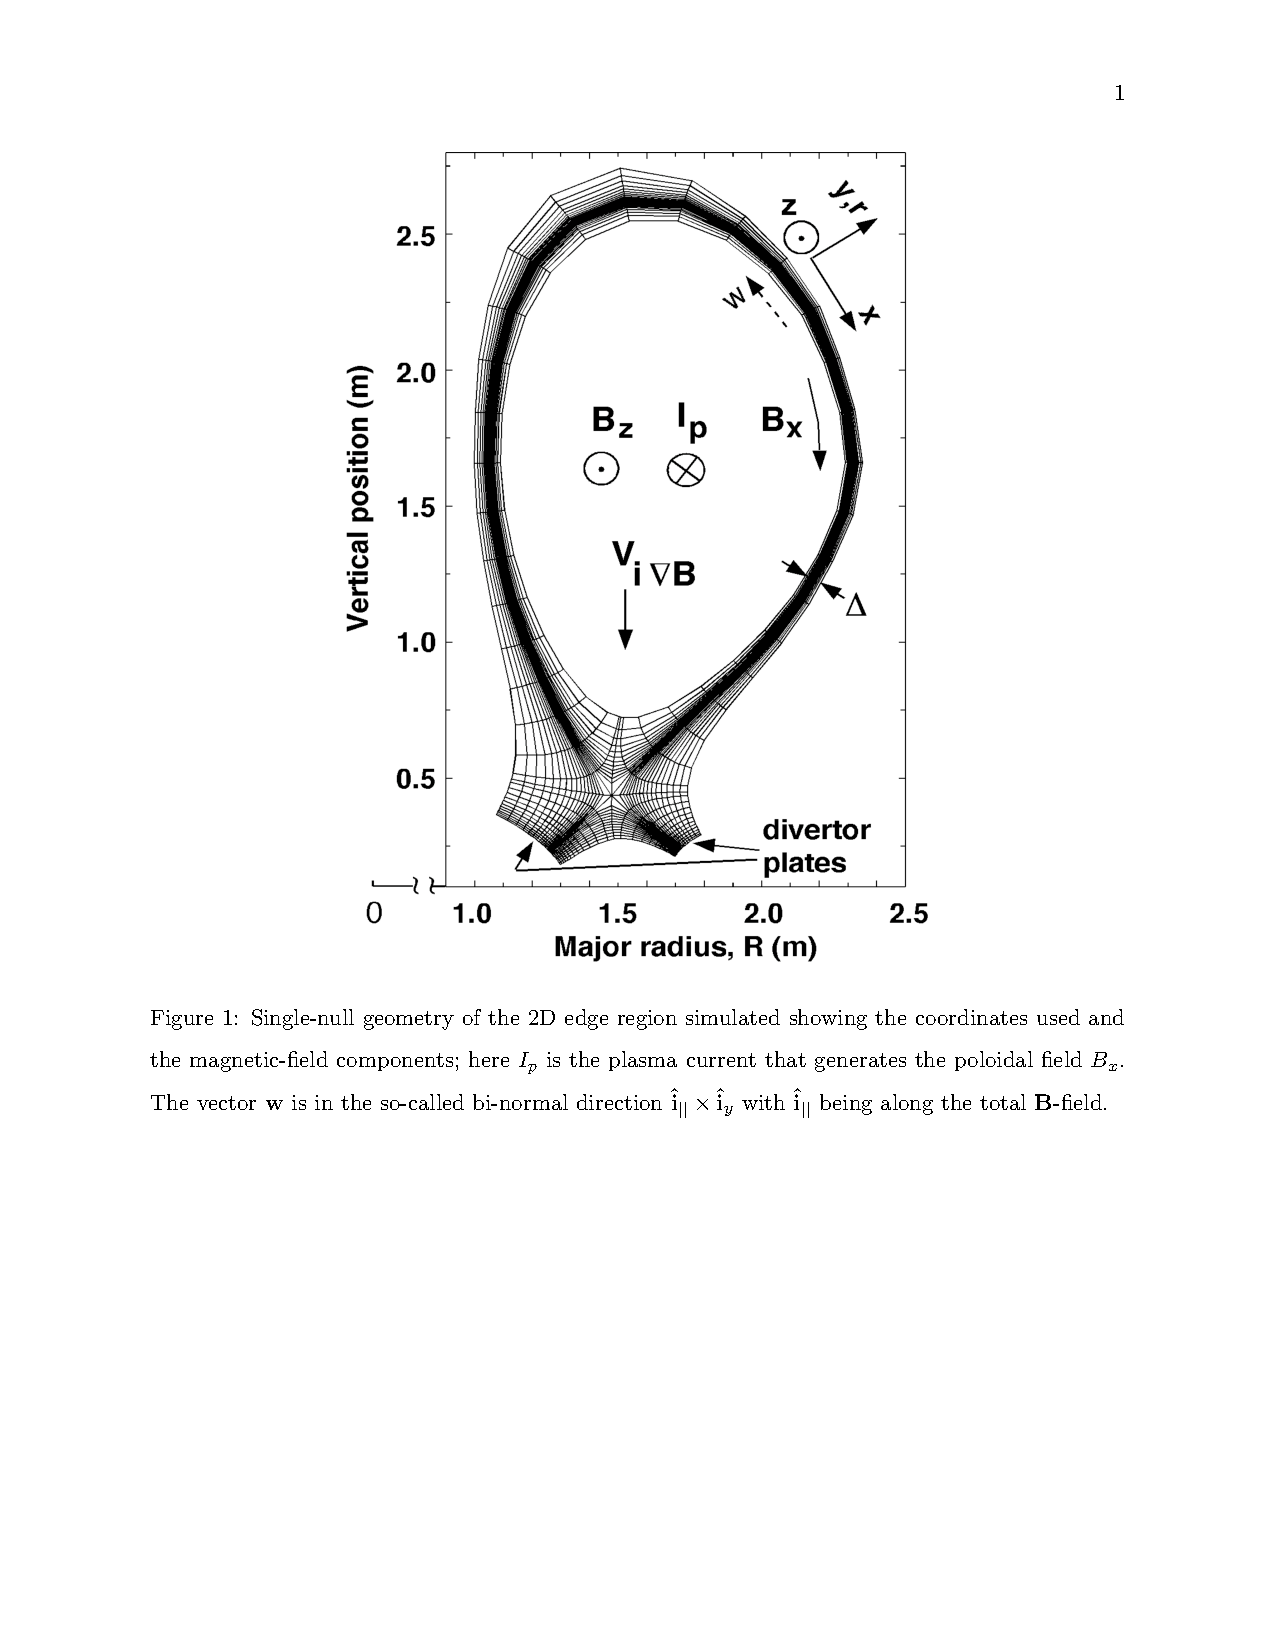
\includepdf[pages=-]{ue_geom_fig_only.pdf}

\section{A Primer on Input Files and Obtaining Initial UEDGE Solutions} 

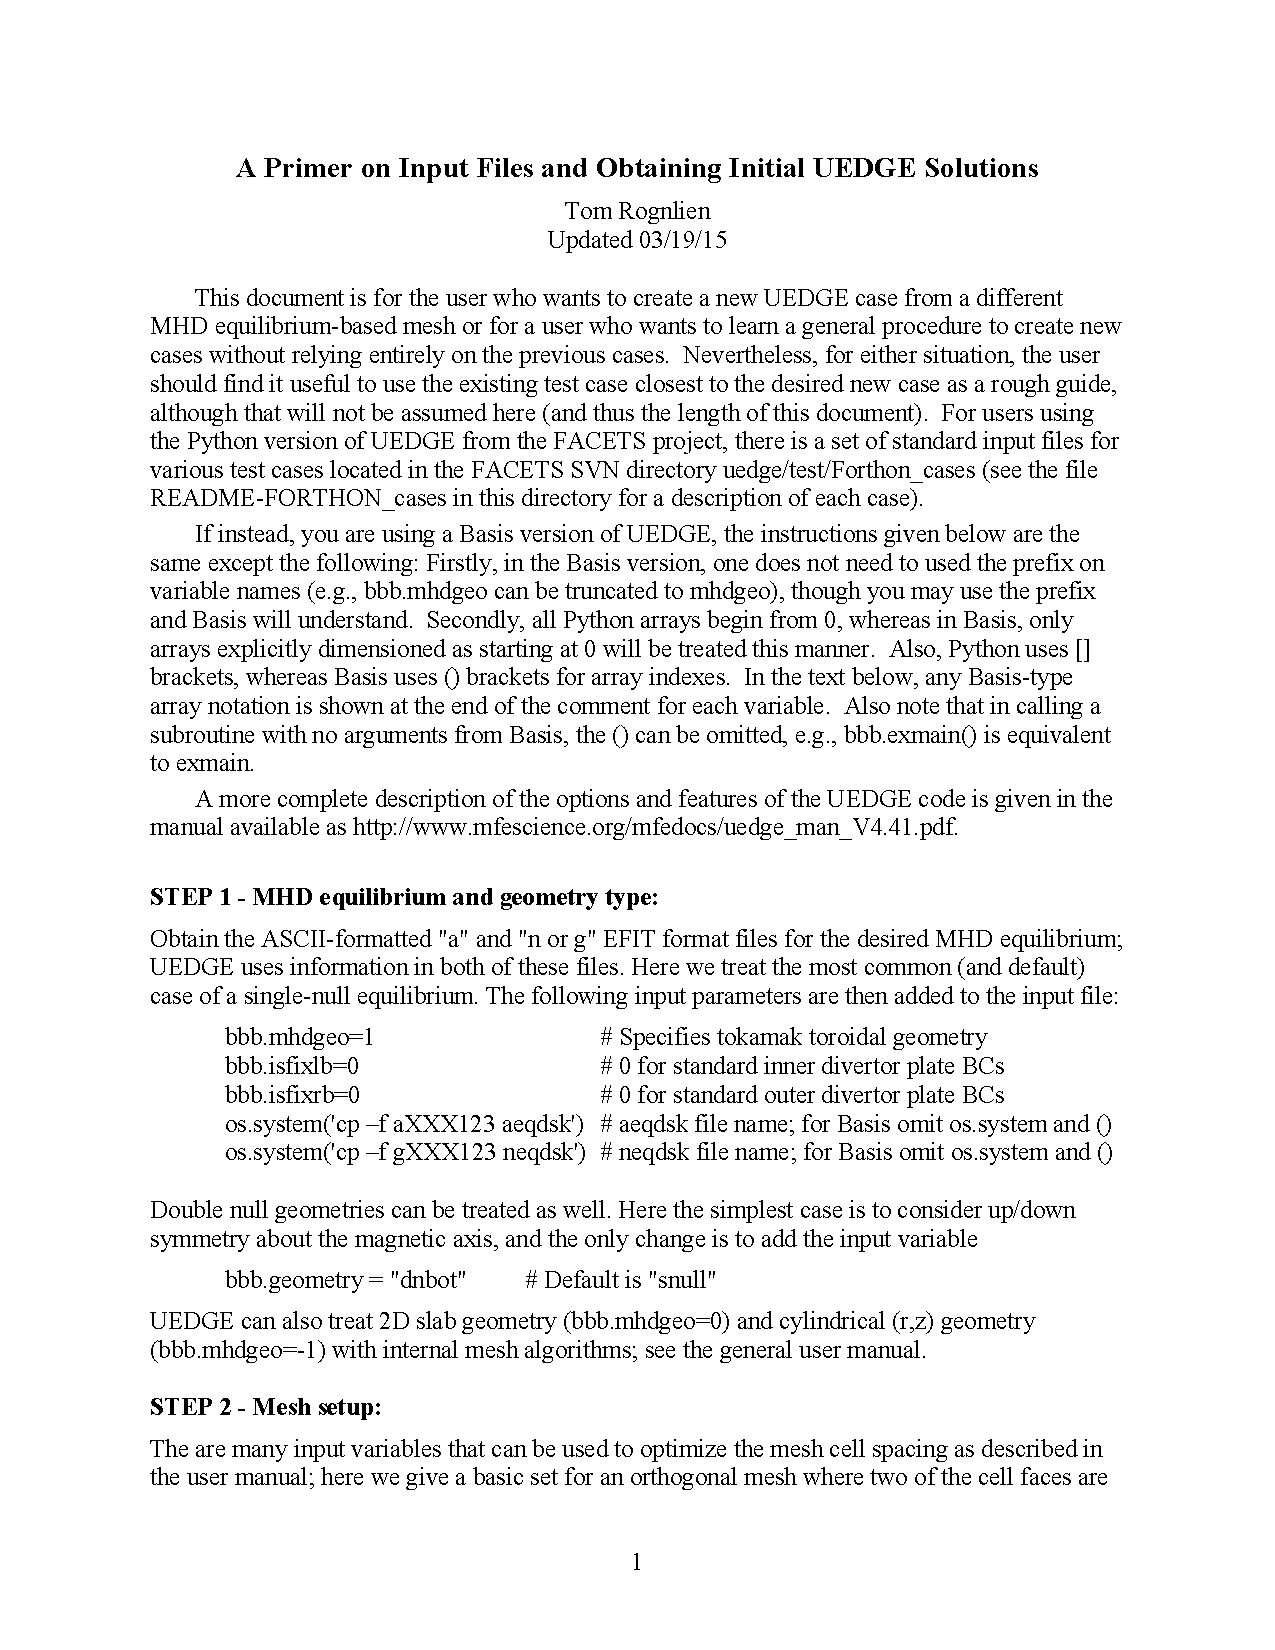
\includepdf[pages=-]{UEDGE_Primer_v4.pdf}


\begin{thebibliography}{99}
  
\bibitem{brag} S.I. Braginskii, Transport processes in a plasma {\it Reviews
    of Plasma Physics}, Vol. I, Ed. M.A. Leontovich (Consultants Bureau, New
  York, 1965), p. 205.
  
\bibitem{rog_ryu99} T.D. Rognlien and D.D. Ryutov, ``Psuedoclassical Transport
Equations for Magnetized Edge-Plasmas in the Slab Approximation,'' Plasma
Phys. Reports {\bf 25}, 943 (1999).

\bibitem{braams87} B.J. Braams, ``A Multi-Fluid Code for Simulation of the
  Edge Plasma in Tokamaks,'' NET Rept. No. 68, Jan., 1987; ``Computational
  studies in tokamak equilibrium and transport'' (thesis, Univ. Utrecht, the
  Netherlands, 1986).
 
\bibitem{braams96} B.J. Braams, ``Radiative Divertor Modeling for ITER and
  TPX,'' Contrib. Plasma Phys. {\bf 36}, 276 (1996).
  
\bibitem{brown86} P.N. Brown and A.C. Hindmarsh, ``Matrix-Free Methods for
Stiff Systems of ODEs,'' SIAM J. Num. Anal. {\bf 23}, 610 (1986).

\bibitem{saad96} Y. Saad, {\it Iterative Methods for Sparse Linear Systems}
  (PWS Pub. Co., Boston, MA, 1996).

\bibitem{r92a} T.D. Rognlien, J L. Milovich, M. E. Rensink, and G.D. Porter,
  ``A Fully Implicit, Time Dependent 2-D Fluid Code for Modeling Tokamak Edge
  Plasmas,'' J. Nucl. Mater. {\bf 196-198}, 347 (1992).
  
\bibitem{r92b} T.D. Rognlien, J.L. Milovich, M.E. Rensink, and T.B.  Kaiser,
  ``Simulation of Tokamak Divertor Plasmas Including Cross-Field Drifts,''
  Contr. Plasma Phys. {\bf 32}, 485 (1992).

\bibitem{p94} G.D. Porter, M. Fenstremacher, R. Groebner, {\it et al.},
  ``Benchmarking UEDGE with DIII-D Data, Contr. Plasma Phys. {\bf 34}, 454
  (1994).
  
\bibitem{r94} T.D. Rognlien, P.N. Brown, R.B. Campbell, {\it et al.}, ``2-D
  Fluid Transport Simulations of Gaseous/Radiative Divertor,'' Contr. Plasma
  Phys.  {\bf 34}, 362 (1994).
  
\bibitem{s95} G.R. Smith, P.N. Brown, R.B. Campbell, {\it et al.},``Techniques
  and Results of Tokamak-Edge Simulation,'' J. Nucl. Mat. {\bf 220-222}, 1024
  (1995).
  
\bibitem{f95} M.E. Fenstermacher, {\it et al.}, ``UEDGE and DEGAS Modeling of
  the DIII-D Scrape-Off Layer Plasma,'' J. Nucl. Mat. {\bf 220-222}, 330
  (1995).
  
\bibitem{p96} G.D. Porter, {\it et al.}, ``Simulation of Experimentally
  Achieved DIII-D Detached Plasmas Using the UEDGE Code,'' Phys. Plasmas {\bf
    3}, 1967 (1996).
  
\bibitem{w96a} F. Wising, D.A. Knoll, S. Krasheninnikov, and T.D. Rognlien,
  ``Simulation of Detachment in ITER-Geometry Using the UEDGE Code and a Fluid
  Neutral Model,'' Contr. Plasma Phys. {\bf  36}, 309 (1996).
  
\bibitem{w96b} F. Wising, D.A. Knoll, S. Krasheninnikov, T.D. Rognlien, and
  D.J. Sigmar, ``Simulation of the Alcator C-Mod Divertor with an Improved
  Neutral Model,'' Contr. Plasma Phys. {\bf  36}, 136 (1996).
  
\bibitem{r96} T.D. Rognlien, B.J. Braams, and D.A. Knoll, ``Progress in
  Integrated 2-D Models for Analysis of Scrape-Off Layer Transport Physics,''
  Contr. Plasma Phys. {\bf  36}, 105 (1996).
  
\bibitem{r97} T.D. Rognlien, J.A. Crotinger, G.D. Porter, {\it et
    al.},``Simulation of the Scrape-Off Layer Plasma During a Disruption,'' J.
  Nucl. Mat. {\bf 241-243}, 590 (1997).

\bibitem{w97} F. Wising, S.I. Krasheninnikov, D.J. Sigmar, D.A. Knoll, T.D.
  Rognlien, B. LaBombard, B. Lipschultz, and G. McCracken, ``Simulation of
  Plasma Flux Detachment in Alcator C-Mod and ITER,'' J. Nucl. Mat. {\bf
    241-243}, 273 (1997).
  
\bibitem{r98a} T.D. Rognlien and D.D. Ryutov, ``Analysis of Classical Transport
  Equations for the Tokamak Edge Plasma,'' Contr. Plasma Phys. {\bf  38}, 152
  (1998).
  
\bibitem{r98b} T.D. Rognlien, D.D. Ryutov, and N. Mattor, ``Calculation of 2-D
  Profiles for the Plasma and Electric Field near a Tokamak Separatrix,''
  Czech. J. Phys. {\bf  48/S2}, 201 (1998).
  
\bibitem{re98} M.E. Rensink, L.L. LoDestro, {\it et al.}, ``A Comparison of
  Neutral Gas Models for Divertor Plasmas,'' Contr. Plasma Phys. {\bf 38}, 325
  (1998).
  
\bibitem{r99a} T.D. Rognlien, G.D. Porter, and D.D. Ryutov, ``Influence of ExB
  and Grad-B Terms in 2-D Edge/SOL Transport Simulations,'' J. Nucl. Mater.
  {\bf 266-269}, 654 (1999).
  
\bibitem{re99a} M.E. Rensink and T.D. Rognlien, ``Edge Plasma Modeling of
  Limiter Surfaces in a Tokamak Divertor Configuration,'' J. Nucl. Mater. {\bf
    266-269}, 1180 (1999).
  
\bibitem{k99} S.I. Krasheninnikov, M.E. Rensink, T.D. Rognlien, {\it et al.},
  ``Stability of the Detachment Front in a Tokamak Divertor,'' J. Nucl. Mater.
  {\bf 266-269}, 251 (1999).

\bibitem{r99} T.D. Rognlien, D.D. Ryutov, N. Mattor, and G.D. Porter,
  ``Two-Dimensional Electric Fields and Drifts near the Magnetic Separatrix in
  Divertor Tokamaks,'' Phys. Plasmas {\bf 6}, 1851 (1999).
  
\bibitem{petravic87} M. Petravic, ``Orthogonal Grid Construction for Modeling
  of Transport in Tokamaks,'' J. Comp. Phys. {\bf 73}, 125 (1987).

\bibitem{byrne92} G.D. Byrne, ``Pragmatic experiments with Krylov methods in
  the stiff ODE setting,'' in {\it Computational Ordinary Differential
    Equations}, edited by J.R. Cash and I. Gladwell, (Oxford Univ. Press,
  Oxford, U.K., 1992) p. 323.
  
\bibitem{brown90} P.N. Brown and Y. Saad, ``Hybrid Krylov methods for
  nonlinear systems of equation,'' SIAM J. Sci. Stat. Comput. {\bf 11}, 450
  (1990).

\bibitem{hindm98} A.C. Hindmarsh and A.G. Taylor, ``{\sf PVODE} and {\sf
    KINSOL}: Parallel software for differential and nonlinear systems,'' Tech.
  Rpt. UCRL-ID-129739, Lawrence Livermore National Lab. (1998).
  
\bibitem{rog_pu} T.D. Rognlien, X.Q. Xu, and A.C. Hindmarsh, ``Application of
  parallel implicit methods to edge-plasma numerical simulations,''J. Comp. Phys.
{\bf 175}, 249 (2002).
  
\bibitem{stotler00} D.P. Stotler, {\it et al.}, ``Coupling of Parallelized
  DEGAS~2 and UEDGE Codes,'' Contr. Plasma Phys. {\bf 40} 221 (2000).
  
\bibitem{stot93} D.P. Stotler, D.E. Post, and D. Reiter, Bull. Am. Phys.  Soc.
  {\bf 38} (1993) 1919; D.P. Stotler, C.S. Pitcher, C.J. Boswell, {\it et
    al.}, J.  Nucl. Mater. {\bf 290-293} 967 (2001). See also the web site
  http://w3.pppl.gov/degas2/.

\bibitem{igit88} Yu.L. Igithanov, Contr. Plasma Phys. {\bf 28}, 477 (1988).
  
\bibitem{keil91} M. Keilhacker, R. Simonini, A. Taroni, and M.L. Watkins,
  Nucl. Fusion {\bf 31}, 535 (1991).

\bibitem{hulse83} R.A. Hulse, Nucl. Tech./Fusion {\bf 3} (1983) 259.
  
\bibitem{behr87} K. Behringer, ``Description of the Impurity Transport Code
  STRAHL,'' JET Report R(87)08 (1987).

\end{thebibliography} 



\end{document}
